\chapter{Experiment 2}
\label{ch:5}
\section{Introduction}

Experiment 1 (Chapter \ref{ch:4}) of the current study investigates the accentedness of various speech patterns in non-native (L2) English speech. The most common native (L1) productions were defined as the L1 target productions. L2 speech that differs from its L1 target production was considered as having mismatches. Results of Experiment 1 show that L2 stimuli with consonant mismatches were judged as being more accented than L2 stimuli with syllable and vowel mismatches. Raters of Experiment 1 did not receive any training before the experiment and were not aware of the intended meaning of each stimulus. These experimental limitations could have affected raters’ accentedness judgments. In addition, sub-phonemic acoustic information of the stimuli was not examined. Questions remain as to whether and how the experimental limitations and sub-phonemic information of the stimuli affected accentedness perception. Experiment 2 of the current study aims to address the potential shortcomings of Experiment 1. 

The same 100 stimuli from Experiment 1 were used in Experiment 2. An additional 150 raters were recruited on Amazon Mechanical Turk (MTurk). In addition to ranking the accentedness of different types of mismatches, Experiment 2 also investigates the effect of sub-phonemic acoustic information on accentedness perception.


\section{Procedure}
To familiarize raters with the full range of accents, a training phase was added at the beginning of the experiment, consisting of ten trials. Ten stimuli were selected for the training phase based on the accentedness ratings collected in Experiment 1. Raters of Experiment 1 judged the accentedness of a stimulus on a 9-point Likert-like scale. Among the ten stimuli, two received the highest accentedness ratings in Experiment 1, two received the lowest ratings, two received an average rating at around 6, two received an average rating at around 5, another two received an average rating at around 4. Table 5.1 illustrates the ten stimuli and their mean accentedness ratings obtained in Experiment 1. To familiarize raters with the five contexts, each context occurred twice during the training phase. The same ten stimuli were used during the training phase for all raters. The presentation of the ten training phase stimuli was randomized for each rater.

% Table generated by Excel2LaTeX from sheet 'exp2train'
\begin{table}[!h]
  \figSpace
  \centering
  \caption{Mean Ratings of the Ten Training Session Stimuli}
    \begin{tabular}{lcll}
    \toprule
     Contexts & Mean Ratings & Types of Stimuli \\
    \midrule
     \textit{please call} & 2.22  & Match \\
     \textit{ask her} & 3.61  & Match \\
   \textit{small plastic} & 3.96  & Vowel Mismatch \\
     \textit{six spoons} & 4.10   & Syllable Mismatch \\
     \textit{five thick} & 4.89  & Vowel Mismatch \\
     \textit{five thick} & 5.07  & Syllable Mismatch \\
    \textit{small plastic} & 5.73  & Syllable Mismatch \\
     \textit{six spoons} & 5.71  & Consonant Mismatch \\
     \textit{please call} & 6.10   & Syllable Mismatch \\
     \textit{ask her} & 7.27  & Consonant Mismatch \\
    \bottomrule
    \end{tabular}%
  \label{tab:train}%
    \figSpace
\end{table}%

To control for the effect of intelligibility, the script of each stimulus was shown on the screen together with the instructions. The raters were instructed to click on a button to hear each stimulus, after which a 9-point Likert-like scale would appear.  Raters then rated the accentedness of the stimulus and moved on to the next trial. 

After the training phase, raters were informed that the actual experiment would begin. This section of the experiment (the testing phase, henceforth) consisted of 100 trials. The presentation of the 100 trials was randomized in the same manner as in Experiment 1. The stimuli used for the testing phase were the same 100 speech samples used for Experiment 1, which included the ten stimuli used for the training phase. After the 100 trials, raters filled out the same demographic questionnaire as in Experiment 1. The maximum time allowed to complete the experiment was 40 minutes. The raters could only listen to each stimulus once. Figure \ref{fig:exp2} demonstrates the interface of the experiment.

\begin{figure}[!h]
  \figSpace
    \centering
	\includegraphics[width=0.75\textwidth]{figures/exp2.jpg}
    \caption{Interface of Experiment 2}
    \label{fig:exp2}
  \figSpace
\end{figure}

\section{Raters}

150 raters were recruited on the MTurk platform. Among the 150 raters, 17 raters self-reported as being an L2 English speaker, or having speech or hearing related problems, or being born outside of the United States. These 17 raters’ responses were excluded from the final analysis. The remaining 133 raters self-reported as L1 English speakers who were born and currently reside in the United States. Among the 133 raters, 68 were male, 58 were female; seven raters did not report their gender\footnote{Some of these raters conveyed to the experimenter their dissatisfaction with the male/female dichotomy implied by the questionnaire.}. The mean age of the 133 raters was 38.42 (SD = 11.84). The raters were from 33 states and the District of Columbia in the continental United States (See Appendix B for rater demographics). The average time for the 133 raters to complete the experiment was 15.96 minutes (SD = 5.47 minutes). All 150 raters were paid \$0.50 for their participation.

\section{Results}
\subsection{Experiment 2: Predictions}

Results of Experiment 1 show that ratings of the 100 stimuli were not consistent over time. Detailed analysis show that raters were making adjustments during the first few trials of the experiment, probably due to their unfamiliarity with the procedure of the experiment and the range of accents. Since Experiment 1 did not inform raters of the intended meaning of each stimulus, intelligibility of the stimuli could have affected raters’ judgment. Experiment 2 accounted for these issues by including a training phase and directly informing raters of the intended meaning of each stimulus. It is, thus, expected that the ratings during the testing phase of Experiment 2 would be more consistent than ratings of Experiment 1. 

Experiment 1 shows that stimuli with consonant mismatches were judged to be more accented than stimuli with vowel and syllable mismatches. Experiment 1 also shows that phonological context potentially affected how accented a stimulus was judged. The same results are expected for Experiment 2. 

\subsection{Segmental and Structural Mismatches}
Ratings from the training phase were excluded from the analysis. Only ratings during the testing phase were analyzed. All the stimuli were rated on a scale from 1 to 9: the larger the number, the more foreign-accented a stimulus was judged. As mentioned in previous chapters, the most common L1 productions in the SAA were considered L1 target productions. 25 of the 100 L2 speech samples were transcribed the same as their respective L1 target productions. These 25 speech samples were termed the match stimuli. IPA transcriptions of the remaining 75 stimuli were not the same as their respective L1 target productions. These 75 stimuli were termed the mismatch stimuli. The mismatch stimuli were further grouped into four types to reflect how they differ from L1 target productions.

There were 5 phonological contexts and 4 types (i.e., consonant vs. vowel vs. syllable vs. match) for the 100 stimuli. There were 20 stimuli for each context, five of which contained only one consonant mismatch, five contained only one vowel mismatch, five contained only one syllable structural mismatch, and another five did not contain any segmental or syllable mismatches (i.e., the match stimuli).


The mean ratings of all of the 100 stimuli was 5.13 (SD=2.29). Raters assigned higher ratings to stimuli with segmental and syllable structural mismatches (M=5.36, SD=2.21) than the match stimuli (M=4.42, SD=2.35). Ratings of stimuli with consonant mismatches (M=5.70, SD=2.11) were on average higher than ratings of stimuli with syllable mismatches (M=5.40, SD=2.29), which was on average higher than stimuli with vowel mismatches (M=5.00, SD=2.18). The general trend is similar to results of Experiment 1. Figure \ref{fig:bar2} demonstrates the mean ratings of each type, where the error bars represent the 95\% confidence intervals.

\begin{figure}[!h]
  \figSpace
\centering
\begin{center}
\begin{tikzpicture}
  \begin{axis}[
  ylabel={Mean Ratings},
width=9.2cm,
   height = 7cm,
    ytick distance=1,
        nodes near coords,
      major x tick style = transparent,
    ybar=3*\pgflinewidth,
      bar width=30pt,
      ymajorgrids = true,
      symbolic x coords={Match,Vowel,Syllable,Consonant},
      xtick ={Match,Vowel, Syllable, Consonant},
      scaled y ticks = false,
        legend style={at={(1.2,0.55)},
  anchor=north},
  legend cell align=left,
      enlarge x limits=0.20,
      ymin=0,
       every axis plot/.append style={
          ybar,
          bar shift=0pt,
          fill
        }
    ]
\addplot [fill=mycolor4,error bars/.cd, y dir=both, y explicit,error bar style=black] 
  coordinates {
          (Match, 4.42) += (0,0.08) -= (0,0.08)};
\addplot [fill=mycolor3,error bars/.cd, y dir=both, y explicit,error bar style=black] 
  coordinates {
          (Vowel, 5.00) += (0,0.08) -= (0,0.08)};
\addplot [fill=mycolor2,error bars/.cd, y dir=both, y explicit,error bar style=black] 
  coordinates {
          (Syllable, 5.40) += (0,0.08) -= (0,0.08)};
 \addplot [fill=mycolor1,error bars/.cd, y dir=both, y explicit,error bar style=black] 
  coordinates {
          (Consonant, 5.70) += (0,0.08) -= (0,0.08)};
  \legend{Match,Vowel,Syllable,Consonant}
 \end{axis}
\end{tikzpicture}
\end{center}



\caption{Mean Ratings by Type of Stimuli on the Scale from 1 to 9}
\label{fig:bar2}
\figSpace
\end{figure}

Linear mixed-effects regression models were employed with the \textit{lme4} package in R \citep{Bates_2014} to investigate segmental and syllable influences on foreign accent perception. The regression models were built the same way as the ones used for Experiment 1. Model comparisons were conducted using the Likelihood Ratio Test as described in Chapter 4. The results show that the DTW scores, which represent prosodic differences between L1 and L2 speech samples, and the interactions involving the DTW scores did not contribute significantly to model fit, showing that prosodic information of the stimuli might not be a major contributing factor to accentedness judgment. 

Just as in Experiment 1, types of stimuli were coded using Helmert contrasts. Results show that the contrast between consonant and syllable mismatches did not achieve significant contribution to model fit (χ2=1.60, p=.21), indicating that ratings of stimuli with consonant and syllable mismatches did not differ significantly from each other. The second contrast, which compared vowel mismatches with consonant and syllable mismatches, contributed significantly to model fit (χ2 = 5.15, p < .02), showing that stimuli with consonant and syllable mismatches were rated as being more accented than stimuli with vowel mismatches. The third contrast, which compares the match stimuli with the three types of mismatch stimuli contributed significantly to model fit (χ2 = 19.84, p < .001), showing that stimuli with mismatches were rated as being more foreign-accented than the match stimuli.

These results suggest that all three types of mismatches contributed to perceived foreign-accentedness. Among the three types of mismatches, vowel mismatches were rated to be the least accented. 

\subsection{Ratings across Time}

Just as in Experiment 1, trial number, which represented time, contributed significantly to model fit (β=0.6, χ2 = 69.91, p < .001), while the interactions between trial number and the three contrasts did not contribute significantly to model fit. These results show that ratings of the four types of stimuli increased over time.

Unlike Experiment 1, Experiment 2 included a training phase, containing ten stimuli covering the range of accents included in the experiment. Ratings obtained by Experiment 1 show that the raters were making adjustments during the first few trials. To investigate whether the inclusion of a training phase and the controlling of intelligibility had affected accentedness judgment, a Smoothing Spline ANOVA (SSANOVA) method was implemented with the \textit{gss} package in R \citep{Gu_2013}. The results are shown in Figure \ref{fig:tr2}, where the solid line represents ratings from Experiment 1 and the dotted line represents ratings from Experiment 2. The shaded areas represent 95\% Bayesian confidence intervals. As Figure \ref{fig:tr2} shows, ratings of Experiment 1 experienced a sudden drop during the first 10 to 15 trials and then the ratings went up. However, ratings obtained by Experiment 2 were more consistent. In other words, no adjustment was observed during the testing phase of Experiment 2. Ratings of Experiment 2 were also generally higher than ratings of Experiment 1.

\begin{figure}[!h]
  \figSpace
    \centering
% Created by tikzDevice version 0.12.3 on 2019-11-25 17:34:11
% !TEX encoding = UTF-8 Unicode
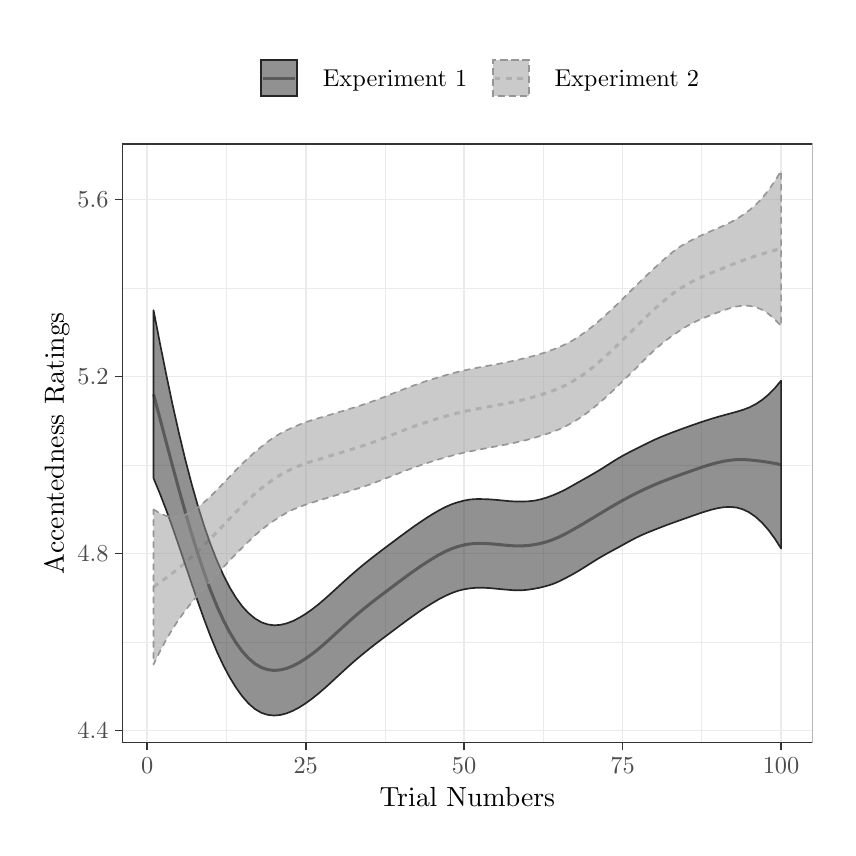
\begin{tikzpicture}[x=1pt,y=1pt]
\definecolor{fillColor}{RGB}{255,255,255}
\path[use as bounding box,fill=fillColor,fill opacity=0.00] (0,0) rectangle (289.08,289.08);
\begin{scope}
\path[clip] (  0.00,  0.00) rectangle (289.08,289.08);
\definecolor{drawColor}{RGB}{255,255,255}
\definecolor{fillColor}{RGB}{255,255,255}

\path[draw=drawColor,line width= 0.6pt,line join=round,line cap=round,fill=fillColor] (  0.00,  0.00) rectangle (289.08,289.08);
\end{scope}
\begin{scope}
\path[clip] ( 34.16, 30.69) rectangle (283.58,247.13);
\definecolor{fillColor}{RGB}{255,255,255}

\path[fill=fillColor] ( 34.16, 30.69) rectangle (283.58,247.13);
\definecolor{drawColor}{gray}{0.92}

\path[draw=drawColor,line width= 0.3pt,line join=round] ( 34.16, 67.10) --
	(283.58, 67.10);

\path[draw=drawColor,line width= 0.3pt,line join=round] ( 34.16,131.06) --
	(283.58,131.06);

\path[draw=drawColor,line width= 0.3pt,line join=round] ( 34.16,195.01) --
	(283.58,195.01);

\path[draw=drawColor,line width= 0.3pt,line join=round] ( 71.83, 30.69) --
	( 71.83,247.13);

\path[draw=drawColor,line width= 0.3pt,line join=round] (129.09, 30.69) --
	(129.09,247.13);

\path[draw=drawColor,line width= 0.3pt,line join=round] (186.35, 30.69) --
	(186.35,247.13);

\path[draw=drawColor,line width= 0.3pt,line join=round] (243.61, 30.69) --
	(243.61,247.13);

\path[draw=drawColor,line width= 0.6pt,line join=round] ( 34.16, 35.13) --
	(283.58, 35.13);

\path[draw=drawColor,line width= 0.6pt,line join=round] ( 34.16, 99.08) --
	(283.58, 99.08);

\path[draw=drawColor,line width= 0.6pt,line join=round] ( 34.16,163.03) --
	(283.58,163.03);

\path[draw=drawColor,line width= 0.6pt,line join=round] ( 34.16,226.99) --
	(283.58,226.99);

\path[draw=drawColor,line width= 0.6pt,line join=round] ( 43.20, 30.69) --
	( 43.20,247.13);

\path[draw=drawColor,line width= 0.6pt,line join=round] (100.46, 30.69) --
	(100.46,247.13);

\path[draw=drawColor,line width= 0.6pt,line join=round] (157.72, 30.69) --
	(157.72,247.13);

\path[draw=drawColor,line width= 0.6pt,line join=round] (214.98, 30.69) --
	(214.98,247.13);

\path[draw=drawColor,line width= 0.6pt,line join=round] (272.24, 30.69) --
	(272.24,247.13);
\definecolor{drawColor}{RGB}{37,37,37}

\path[draw=drawColor,draw opacity=0.50,line width= 1.1pt,line join=round] ( 45.49,156.60) --
	( 47.78,147.92) --
	( 50.07,139.25) --
	( 52.36,130.63) --
	( 54.66,122.19) --
	( 56.95,114.02) --
	( 59.24,106.21) --
	( 61.53, 98.84) --
	( 63.82, 91.98) --
	( 66.11, 85.68) --
	( 68.40, 80.02) --
	( 70.69, 75.00) --
	( 72.98, 70.61) --
	( 75.27, 66.84) --
	( 77.56, 63.69) --
	( 79.85, 61.16) --
	( 82.14, 59.22) --
	( 84.43, 57.88) --
	( 86.72, 57.10) --
	( 89.01, 56.83) --
	( 91.30, 57.00) --
	( 93.59, 57.57) --
	( 95.88, 58.47) --
	( 98.17, 59.67) --
	(100.46, 61.10) --
	(102.75, 62.75) --
	(105.04, 64.56) --
	(107.33, 66.51) --
	(109.62, 68.57) --
	(111.91, 70.69) --
	(114.21, 72.80) --
	(116.50, 74.86) --
	(118.79, 76.86) --
	(121.08, 78.78) --
	(123.37, 80.63) --
	(125.66, 82.42) --
	(127.95, 84.17) --
	(130.24, 85.88) --
	(132.53, 87.60) --
	(134.82, 89.32) --
	(137.11, 91.01) --
	(139.40, 92.66) --
	(141.69, 94.26) --
	(143.98, 95.78) --
	(146.27, 97.23) --
	(148.56, 98.57) --
	(150.85, 99.77) --
	(153.14,100.78) --
	(155.43,101.58) --
	(157.72,102.17) --
	(160.01,102.55) --
	(162.30,102.72) --
	(164.59,102.72) --
	(166.88,102.60) --
	(169.17,102.41) --
	(171.47,102.19) --
	(173.76,101.97) --
	(176.05,101.82) --
	(178.34,101.80) --
	(180.63,101.94) --
	(182.92,102.23) --
	(185.21,102.68) --
	(187.50,103.30) --
	(189.79,104.09) --
	(192.08,105.06) --
	(194.37,106.20) --
	(196.66,107.45) --
	(198.95,108.76) --
	(201.24,110.11) --
	(203.53,111.48) --
	(205.82,112.87) --
	(208.11,114.25) --
	(210.40,115.62) --
	(212.69,116.96) --
	(214.98,118.25) --
	(217.27,119.49) --
	(219.56,120.67) --
	(221.85,121.80) --
	(224.14,122.86) --
	(226.43,123.88) --
	(228.73,124.83) --
	(231.02,125.73) --
	(233.31,126.59) --
	(235.60,127.42) --
	(237.89,128.24) --
	(240.18,129.05) --
	(242.47,129.85) --
	(244.76,130.61) --
	(247.05,131.32) --
	(249.34,131.93) --
	(251.63,132.43) --
	(253.92,132.79) --
	(256.21,132.99) --
	(258.50,133.01) --
	(260.79,132.88) --
	(263.08,132.66) --
	(265.37,132.37) --
	(267.66,132.03) --
	(269.95,131.63) --
	(272.24,131.19);
\definecolor{drawColor}{RGB}{150,150,150}

\path[draw=drawColor,draw opacity=0.50,line width= 1.1pt,dash pattern=on 2pt off 2pt ,line join=round] ( 45.49, 87.00) --
	( 47.78, 88.64) --
	( 50.07, 90.32) --
	( 52.36, 92.03) --
	( 54.66, 93.84) --
	( 56.95, 95.76) --
	( 59.24, 97.78) --
	( 61.53, 99.92) --
	( 63.82,102.15) --
	( 66.11,104.47) --
	( 68.40,106.85) --
	( 70.69,109.26) --
	( 72.98,111.68) --
	( 75.27,114.06) --
	( 77.56,116.37) --
	( 79.85,118.58) --
	( 82.14,120.67) --
	( 84.43,122.62) --
	( 86.72,124.41) --
	( 89.01,126.03) --
	( 91.30,127.45) --
	( 93.59,128.71) --
	( 95.88,129.81) --
	( 98.17,130.77) --
	(100.46,131.62) --
	(102.75,132.38) --
	(105.04,133.07) --
	(107.33,133.75) --
	(109.62,134.43) --
	(111.91,135.12) --
	(114.21,135.82) --
	(116.50,136.53) --
	(118.79,137.25) --
	(121.08,137.99) --
	(123.37,138.77) --
	(125.66,139.60) --
	(127.95,140.47) --
	(130.24,141.37) --
	(132.53,142.28) --
	(134.82,143.19) --
	(137.11,144.07) --
	(139.40,144.92) --
	(141.69,145.72) --
	(143.98,146.49) --
	(146.27,147.23) --
	(148.56,147.94) --
	(150.85,148.61) --
	(153.14,149.24) --
	(155.43,149.83) --
	(157.72,150.37) --
	(160.01,150.86) --
	(162.30,151.31) --
	(164.59,151.74) --
	(166.88,152.17) --
	(169.17,152.59) --
	(171.47,153.02) --
	(173.76,153.48) --
	(176.05,153.95) --
	(178.34,154.47) --
	(180.63,155.04) --
	(182.92,155.67) --
	(185.21,156.34) --
	(187.50,157.08) --
	(189.79,157.90) --
	(192.08,158.81) --
	(194.37,159.87) --
	(196.66,161.10) --
	(198.95,162.50) --
	(201.24,164.07) --
	(203.53,165.81) --
	(205.82,167.69) --
	(208.11,169.69) --
	(210.40,171.78) --
	(212.69,173.94) --
	(214.98,176.16) --
	(217.27,178.42) --
	(219.56,180.70) --
	(221.85,182.96) --
	(224.14,185.18) --
	(226.43,187.34) --
	(228.73,189.39) --
	(231.02,191.33) --
	(233.31,193.11) --
	(235.60,194.72) --
	(237.89,196.13) --
	(240.18,197.37) --
	(242.47,198.48) --
	(244.76,199.50) --
	(247.05,200.46) --
	(249.34,201.39) --
	(251.63,202.31) --
	(253.92,203.23) --
	(256.21,204.15) --
	(258.50,205.02) --
	(260.79,205.84) --
	(263.08,206.59) --
	(265.37,207.31) --
	(267.66,207.98) --
	(269.95,208.64) --
	(272.24,209.28);
\definecolor{drawColor}{RGB}{37,37,37}
\definecolor{fillColor}{RGB}{37,37,37}

\path[draw=drawColor,line width= 0.6pt,line join=round,line cap=round,fill=fillColor,fill opacity=0.50] ( 45.49,186.96) --
	( 47.78,175.12) --
	( 50.07,163.72) --
	( 52.36,152.84) --
	( 54.66,142.58) --
	( 56.95,133.04) --
	( 59.24,124.23) --
	( 61.53,116.17) --
	( 63.82,108.85) --
	( 66.11,102.31) --
	( 68.40, 96.50) --
	( 70.69, 91.34) --
	( 72.98, 86.86) --
	( 75.27, 83.07) --
	( 77.56, 79.95) --
	( 79.85, 77.48) --
	( 82.14, 75.59) --
	( 84.43, 74.23) --
	( 86.72, 73.44) --
	( 89.01, 73.13) --
	( 91.30, 73.28) --
	( 93.59, 73.82) --
	( 95.88, 74.69) --
	( 98.17, 75.86) --
	(100.46, 77.27) --
	(102.75, 78.88) --
	(105.04, 80.67) --
	(107.33, 82.62) --
	(109.62, 84.67) --
	(111.91, 86.77) --
	(114.21, 88.88) --
	(116.50, 90.92) --
	(118.79, 92.92) --
	(121.08, 94.85) --
	(123.37, 96.69) --
	(125.66, 98.47) --
	(127.95,100.23) --
	(130.24,101.94) --
	(132.53,103.65) --
	(134.82,105.37) --
	(137.11,107.06) --
	(139.40,108.72) --
	(141.69,110.30) --
	(143.98,111.83) --
	(146.27,113.28) --
	(148.56,114.62) --
	(150.85,115.83) --
	(153.14,116.82) --
	(155.43,117.59) --
	(157.72,118.20) --
	(160.01,118.61) --
	(162.30,118.75) --
	(164.59,118.73) --
	(166.88,118.64) --
	(169.17,118.46) --
	(171.47,118.24) --
	(173.76,118.01) --
	(176.05,117.87) --
	(178.34,117.84) --
	(180.63,117.91) --
	(182.92,118.14) --
	(185.21,118.60) --
	(187.50,119.27) --
	(189.79,120.12) --
	(192.08,121.10) --
	(194.37,122.21) --
	(196.66,123.49) --
	(198.95,124.80) --
	(201.24,126.08) --
	(203.53,127.37) --
	(205.82,128.71) --
	(208.11,130.13) --
	(210.40,131.59) --
	(212.69,133.04) --
	(214.98,134.38) --
	(217.27,135.59) --
	(219.56,136.73) --
	(221.85,137.88) --
	(224.14,139.03) --
	(226.43,140.14) --
	(228.73,141.14) --
	(231.02,142.07) --
	(233.31,142.96) --
	(235.60,143.80) --
	(237.89,144.64) --
	(240.18,145.45) --
	(242.47,146.24) --
	(244.76,147.01) --
	(247.05,147.74) --
	(249.34,148.42) --
	(251.63,149.06) --
	(253.92,149.67) --
	(256.21,150.30) --
	(258.50,151.00) --
	(260.79,151.87) --
	(263.08,153.04) --
	(265.37,154.56) --
	(267.66,156.46) --
	(269.95,158.78) --
	(272.24,161.52) --
	(272.24,100.87) --
	(269.95,104.48) --
	(267.66,107.59) --
	(265.37,110.19) --
	(263.08,112.28) --
	(260.79,113.89) --
	(258.50,115.01) --
	(256.21,115.67) --
	(253.92,115.91) --
	(251.63,115.81) --
	(249.34,115.45) --
	(247.05,114.89) --
	(244.76,114.21) --
	(242.47,113.45) --
	(240.18,112.66) --
	(237.89,111.85) --
	(235.60,111.05) --
	(233.31,110.22) --
	(231.02,109.39) --
	(228.73,108.52) --
	(226.43,107.61) --
	(224.14,106.70) --
	(221.85,105.72) --
	(219.56,104.62) --
	(217.27,103.40) --
	(214.98,102.13) --
	(212.69,100.88) --
	(210.40, 99.65) --
	(208.11, 98.37) --
	(205.82, 97.02) --
	(203.53, 95.59) --
	(201.24, 94.13) --
	(198.95, 92.72) --
	(196.66, 91.41) --
	(194.37, 90.18) --
	(192.08, 89.02) --
	(189.79, 88.06) --
	(187.50, 87.33) --
	(185.21, 86.76) --
	(182.92, 86.31) --
	(180.63, 85.96) --
	(178.34, 85.77) --
	(176.05, 85.77) --
	(173.76, 85.94) --
	(171.47, 86.14) --
	(169.17, 86.36) --
	(166.88, 86.57) --
	(164.59, 86.71) --
	(162.30, 86.69) --
	(160.01, 86.50) --
	(157.72, 86.14) --
	(155.43, 85.57) --
	(153.14, 84.74) --
	(150.85, 83.72) --
	(148.56, 82.53) --
	(146.27, 81.17) --
	(143.98, 79.74) --
	(141.69, 78.22) --
	(139.40, 76.61) --
	(137.11, 74.96) --
	(134.82, 73.26) --
	(132.53, 71.54) --
	(130.24, 69.83) --
	(127.95, 68.11) --
	(125.66, 66.37) --
	(123.37, 64.57) --
	(121.08, 62.72) --
	(118.79, 60.81) --
	(116.50, 58.81) --
	(114.21, 56.72) --
	(111.91, 54.61) --
	(109.62, 52.48) --
	(107.33, 50.40) --
	(105.04, 48.44) --
	(102.75, 46.61) --
	(100.46, 44.94) --
	( 98.17, 43.47) --
	( 95.88, 42.26) --
	( 93.59, 41.32) --
	( 91.30, 40.72) --
	( 89.01, 40.52) --
	( 86.72, 40.77) --
	( 84.43, 41.52) --
	( 82.14, 42.85) --
	( 79.85, 44.83) --
	( 77.56, 47.43) --
	( 75.27, 50.62) --
	( 72.98, 54.35) --
	( 70.69, 58.65) --
	( 68.40, 63.55) --
	( 66.11, 69.06) --
	( 63.82, 75.10) --
	( 61.53, 81.51) --
	( 59.24, 88.20) --
	( 56.95, 95.00) --
	( 54.66,101.79) --
	( 52.36,108.42) --
	( 50.07,114.78) --
	( 47.78,120.71) --
	( 45.49,126.25) --
	cycle;
\definecolor{drawColor}{gray}{0.59}
\definecolor{fillColor}{RGB}{150,150,150}

\path[draw=drawColor,line width= 0.6pt,dash pattern=on 2pt off 2pt ,line join=round,line cap=round,fill=fillColor,fill opacity=0.50] ( 45.49,115.03) --
	( 47.78,113.59) --
	( 50.07,112.65) --
	( 52.36,112.24) --
	( 54.66,112.37) --
	( 56.95,113.04) --
	( 59.24,114.20) --
	( 61.53,115.76) --
	( 63.82,117.65) --
	( 66.11,119.76) --
	( 68.40,122.05) --
	( 70.69,124.44) --
	( 72.98,126.82) --
	( 75.27,129.20) --
	( 77.56,131.53) --
	( 79.85,133.70) --
	( 82.14,135.72) --
	( 84.43,137.64) --
	( 86.72,139.45) --
	( 89.01,141.09) --
	( 91.30,142.45) --
	( 93.59,143.61) --
	( 95.88,144.66) --
	( 98.17,145.64) --
	(100.46,146.53) --
	(102.75,147.28) --
	(105.04,147.96) --
	(107.33,148.62) --
	(109.62,149.29) --
	(111.91,149.99) --
	(114.21,150.67) --
	(116.50,151.39) --
	(118.79,152.08) --
	(121.08,152.82) --
	(123.37,153.62) --
	(125.66,154.42) --
	(127.95,155.27) --
	(130.24,156.20) --
	(132.53,157.13) --
	(134.82,158.03) --
	(137.11,158.93) --
	(139.40,159.76) --
	(141.69,160.57) --
	(143.98,161.35) --
	(146.27,162.07) --
	(148.56,162.78) --
	(150.85,163.46) --
	(153.14,164.09) --
	(155.43,164.68) --
	(157.72,165.22) --
	(160.01,165.71) --
	(162.30,166.15) --
	(164.59,166.59) --
	(166.88,167.00) --
	(169.17,167.40) --
	(171.47,167.86) --
	(173.76,168.33) --
	(176.05,168.80) --
	(178.34,169.32) --
	(180.63,169.90) --
	(182.92,170.50) --
	(185.21,171.16) --
	(187.50,171.92) --
	(189.79,172.75) --
	(192.08,173.66) --
	(194.37,174.71) --
	(196.66,175.91) --
	(198.95,177.33) --
	(201.24,178.92) --
	(203.53,180.65) --
	(205.82,182.54) --
	(208.11,184.55) --
	(210.40,186.65) --
	(212.69,188.80) --
	(214.98,191.02) --
	(217.27,193.33) --
	(219.56,195.62) --
	(221.85,197.83) --
	(224.14,200.00) --
	(226.43,202.14) --
	(228.73,204.26) --
	(231.02,206.30) --
	(233.31,208.20) --
	(235.60,209.85) --
	(237.89,211.22) --
	(240.18,212.42) --
	(242.47,213.56) --
	(244.76,214.63) --
	(247.05,215.63) --
	(249.34,216.60) --
	(251.63,217.61) --
	(253.92,218.71) --
	(256.21,219.96) --
	(258.50,221.43) --
	(260.79,223.11) --
	(263.08,225.07) --
	(265.37,227.44) --
	(267.66,230.28) --
	(269.95,233.58) --
	(272.24,237.29) --
	(272.24,181.28) --
	(269.95,183.70) --
	(267.66,185.69) --
	(265.37,187.17) --
	(263.08,188.11) --
	(260.79,188.56) --
	(258.50,188.62) --
	(256.21,188.34) --
	(253.92,187.76) --
	(251.63,187.01) --
	(249.34,186.18) --
	(247.05,185.29) --
	(244.76,184.36) --
	(242.47,183.40) --
	(240.18,182.32) --
	(237.89,181.04) --
	(235.60,179.59) --
	(233.31,178.03) --
	(231.02,176.36) --
	(228.73,174.53) --
	(226.43,172.53) --
	(224.14,170.36) --
	(221.85,168.08) --
	(219.56,165.77) --
	(217.27,163.51) --
	(214.98,161.30) --
	(212.69,159.08) --
	(210.40,156.90) --
	(208.11,154.82) --
	(205.82,152.85) --
	(203.53,150.97) --
	(201.24,149.22) --
	(198.95,147.67) --
	(196.66,146.29) --
	(194.37,145.04) --
	(192.08,143.96) --
	(189.79,143.05) --
	(187.50,142.25) --
	(185.21,141.53) --
	(182.92,140.83) --
	(180.63,140.19) --
	(178.34,139.63) --
	(176.05,139.10) --
	(173.76,138.62) --
	(171.47,138.19) --
	(169.17,137.78) --
	(166.88,137.33) --
	(164.59,136.89) --
	(162.30,136.47) --
	(160.01,136.01) --
	(157.72,135.52) --
	(155.43,134.99) --
	(153.14,134.39) --
	(150.85,133.76) --
	(148.56,133.10) --
	(146.27,132.39) --
	(143.98,131.64) --
	(141.69,130.87) --
	(139.40,130.07) --
	(137.11,129.22) --
	(134.82,128.35) --
	(132.53,127.43) --
	(130.24,126.54) --
	(127.95,125.66) --
	(125.66,124.77) --
	(123.37,123.92) --
	(121.08,123.16) --
	(118.79,122.41) --
	(116.50,121.67) --
	(114.21,120.97) --
	(111.91,120.26) --
	(109.62,119.58) --
	(107.33,118.88) --
	(105.04,118.18) --
	(102.75,117.47) --
	(100.46,116.71) --
	( 98.17,115.90) --
	( 95.88,114.95) --
	( 93.59,113.81) --
	( 91.30,112.46) --
	( 89.01,110.97) --
	( 86.72,109.36) --
	( 84.43,107.59) --
	( 82.14,105.61) --
	( 79.85,103.45) --
	( 77.56,101.20) --
	( 75.27, 98.92) --
	( 72.98, 96.53) --
	( 70.69, 94.08) --
	( 68.40, 91.65) --
	( 66.11, 89.17) --
	( 63.82, 86.64) --
	( 61.53, 84.07) --
	( 59.24, 81.36) --
	( 56.95, 78.47) --
	( 54.66, 75.31) --
	( 52.36, 71.83) --
	( 50.07, 67.98) --
	( 47.78, 63.70) --
	( 45.49, 58.97) --
	cycle;
\definecolor{drawColor}{gray}{0.20}

\path[draw=drawColor,line width= 0.6pt,line join=round,line cap=round] ( 34.16, 30.69) rectangle (283.58,247.13);
\end{scope}
\begin{scope}
\path[clip] (  0.00,  0.00) rectangle (289.08,289.08);
\definecolor{drawColor}{gray}{0.30}

\node[text=drawColor,anchor=base east,inner sep=0pt, outer sep=0pt, scale=  0.88] at ( 29.21, 32.10) {4.4};

\node[text=drawColor,anchor=base east,inner sep=0pt, outer sep=0pt, scale=  0.88] at ( 29.21, 96.05) {4.8};

\node[text=drawColor,anchor=base east,inner sep=0pt, outer sep=0pt, scale=  0.88] at ( 29.21,160.00) {5.2};

\node[text=drawColor,anchor=base east,inner sep=0pt, outer sep=0pt, scale=  0.88] at ( 29.21,223.96) {5.6};
\end{scope}
\begin{scope}
\path[clip] (  0.00,  0.00) rectangle (289.08,289.08);
\definecolor{drawColor}{gray}{0.20}

\path[draw=drawColor,line width= 0.6pt,line join=round] ( 31.41, 35.13) --
	( 34.16, 35.13);

\path[draw=drawColor,line width= 0.6pt,line join=round] ( 31.41, 99.08) --
	( 34.16, 99.08);

\path[draw=drawColor,line width= 0.6pt,line join=round] ( 31.41,163.03) --
	( 34.16,163.03);

\path[draw=drawColor,line width= 0.6pt,line join=round] ( 31.41,226.99) --
	( 34.16,226.99);
\end{scope}
\begin{scope}
\path[clip] (  0.00,  0.00) rectangle (289.08,289.08);
\definecolor{drawColor}{gray}{0.20}

\path[draw=drawColor,line width= 0.6pt,line join=round] ( 43.20, 27.94) --
	( 43.20, 30.69);

\path[draw=drawColor,line width= 0.6pt,line join=round] (100.46, 27.94) --
	(100.46, 30.69);

\path[draw=drawColor,line width= 0.6pt,line join=round] (157.72, 27.94) --
	(157.72, 30.69);

\path[draw=drawColor,line width= 0.6pt,line join=round] (214.98, 27.94) --
	(214.98, 30.69);

\path[draw=drawColor,line width= 0.6pt,line join=round] (272.24, 27.94) --
	(272.24, 30.69);
\end{scope}
\begin{scope}
\path[clip] (  0.00,  0.00) rectangle (289.08,289.08);
\definecolor{drawColor}{gray}{0.30}

\node[text=drawColor,anchor=base,inner sep=0pt, outer sep=0pt, scale=  0.88] at ( 43.20, 19.68) {0};

\node[text=drawColor,anchor=base,inner sep=0pt, outer sep=0pt, scale=  0.88] at (100.46, 19.68) {25};

\node[text=drawColor,anchor=base,inner sep=0pt, outer sep=0pt, scale=  0.88] at (157.72, 19.68) {50};

\node[text=drawColor,anchor=base,inner sep=0pt, outer sep=0pt, scale=  0.88] at (214.98, 19.68) {75};

\node[text=drawColor,anchor=base,inner sep=0pt, outer sep=0pt, scale=  0.88] at (272.24, 19.68) {100};
\end{scope}
\begin{scope}
\path[clip] (  0.00,  0.00) rectangle (289.08,289.08);
\definecolor{drawColor}{RGB}{0,0,0}

\node[text=drawColor,anchor=base,inner sep=0pt, outer sep=0pt, scale=  1.00] at (158.87,  7.64) {Trial Numbers};
\end{scope}
\begin{scope}
\path[clip] (  0.00,  0.00) rectangle (289.08,289.08);
\definecolor{drawColor}{RGB}{0,0,0}

\node[text=drawColor,rotate= 90.00,anchor=base,inner sep=0pt, outer sep=0pt, scale=  1.00] at ( 13.08,138.91) {Accentedness Ratings};
\end{scope}
\begin{scope}
\path[clip] (  0.00,  0.00) rectangle (289.08,289.08);
\definecolor{fillColor}{RGB}{255,255,255}

\path[fill=fillColor] ( 69.64,258.13) rectangle (248.09,283.58);
\end{scope}
\begin{scope}
\path[clip] (  0.00,  0.00) rectangle (289.08,289.08);
\definecolor{fillColor}{RGB}{255,255,255}

\path[fill=fillColor] ( 83.68,263.63) rectangle ( 98.13,278.08);
\end{scope}
\begin{scope}
\path[clip] (  0.00,  0.00) rectangle (289.08,289.08);
\definecolor{drawColor}{RGB}{37,37,37}

\path[draw=drawColor,draw opacity=0.50,line width= 1.1pt,line join=round] ( 85.12,270.85) -- ( 96.69,270.85);
\end{scope}
\begin{scope}
\path[clip] (  0.00,  0.00) rectangle (289.08,289.08);
\definecolor{drawColor}{RGB}{37,37,37}
\definecolor{fillColor}{RGB}{37,37,37}

\path[draw=drawColor,line width= 0.6pt,line cap=rect,fill=fillColor,fill opacity=0.50] ( 84.39,264.34) rectangle ( 97.42,277.37);
\end{scope}
\begin{scope}
\path[clip] (  0.00,  0.00) rectangle (289.08,289.08);
\definecolor{fillColor}{RGB}{255,255,255}

\path[fill=fillColor] (167.40,263.63) rectangle (181.86,278.08);
\end{scope}
\begin{scope}
\path[clip] (  0.00,  0.00) rectangle (289.08,289.08);
\definecolor{drawColor}{RGB}{150,150,150}

\path[draw=drawColor,draw opacity=0.50,line width= 1.1pt,dash pattern=on 2pt off 2pt ,line join=round] (168.85,270.85) -- (180.41,270.85);
\end{scope}
\begin{scope}
\path[clip] (  0.00,  0.00) rectangle (289.08,289.08);
\definecolor{drawColor}{gray}{0.59}
\definecolor{fillColor}{RGB}{150,150,150}

\path[draw=drawColor,line width= 0.6pt,dash pattern=on 2pt off 2pt ,line cap=rect,fill=fillColor,fill opacity=0.50] (168.12,264.34) rectangle (181.15,277.37);
\end{scope}
\begin{scope}
\path[clip] (  0.00,  0.00) rectangle (289.08,289.08);
\definecolor{drawColor}{RGB}{0,0,0}

\node[text=drawColor,anchor=base west,inner sep=0pt, outer sep=0pt, scale=  0.88] at (106.67,267.82) {Experiment 1};
\end{scope}
\begin{scope}
\path[clip] (  0.00,  0.00) rectangle (289.08,289.08);
\definecolor{drawColor}{RGB}{0,0,0}

\node[text=drawColor,anchor=base west,inner sep=0pt, outer sep=0pt, scale=  0.88] at (190.39,267.82) {Experiment 2};
\end{scope}
\end{tikzpicture}

    \caption{Ratings across Time (Experiment 1 and Experiment 2)}
    \label{fig:tr2}
  \figSpace
\end{figure}

The ten training phase stimuli were also used in the testing phase.  It is possible that the raters' judgments on these ten stimuli during the testing phase are different from their judgments on other stimuli, simply because the ten stimuli were heard during the training phase. Linear mixed-effects model was run to investigate whether ratings on the ten stimuli during the testing phase are different from ratings on the remaining 90 stimuli. The ratings were the dependent variable.The times a stimulus was heard (once vs. twice), the four types of stimuli, trial number and the interactions between these factors were included as fixed effects. The raters and the stimuli were entered as two random effects. The results show that the times a stimulus was heard did not contribute significantly to model fit (χ2 = 0.01, p = .93). Therefore, ratings of the ten stimuli during the testing phase might not have been affected by the fact that the ten stimuli were included the training phase.


\subsection{Individual Mismatches}

The analysis above focuses on broad categories such as consonant, vowel, and syllable mismatches. However, there were 11 types of consonant mismatches, five types of vowel mismatches and two types of syllable mismatches involved in the experiment. Although consonant mismatches appeared in general to be more accented than the other two types of mismatches, it might be too hasty to draw the conclusion that all consonant mismatches are more accented than the other two types. This section presents a more detailed analysis, which focuses on individual mismatches within a given phonological context. The following section first discusses the statistical methods using one phonological context as an example. Since statistical methods used for the other four phonological contexts are the same as methods used for the first context, the details for these four contexts are omitted. 

\subsubsection{Context 1: “\textit{Ask her}”}

For the context “\textit{ask her},” syllable mismatches such as consonant deletion (i.e., [æsk]$\rightarrow$[æs]) and vowel epenthesis (i.e., [æsk]$\rightarrow$[æskə]) received the highest ratings (i.e., most accented), while vowel mismatches received relatively lower ratings. Figure \ref{fig:ah2} demonstrates the mean ratings of the seven individual mismatches and the match stimuli, where the error bars represent 95\% confidence intervals. 

\begin{figure}[!h]
  \figSpace
\centering

\begin{tikzpicture}
  \begin{axis}[
  title={Mean Accentedness Ratings},
     % xbar,
   ytick={1,2,3,4,5,6,7,8},
     y=1cm,
  bar width=0.7 cm,
  xmin=0,
  xmax=7.1,
    axis y line*=left,
   axis x line=bottom,
    tickwidth         = 1pt,
    enlarge y limits  = 0.1,
    enlarge x limits  = 0.02,
  legend style={at={(1.2,0.55)},
  anchor=north},
  legend cell align=left,
      yticklabels from table={figures/sup/data_askher.txt}{label},
      xtick distance=2,
      every axis plot/.append style={
          xbar,
          bar shift=0pt,
          fill
        }
    ]
\addplot [fill=red,color=mycolor3,select coords between index={0}{0}] table  [x=x,y=y] {figures/sup/data_askher.txt};
\addplot [fill=red,color=mycolor1,select coords between index={1}{1}] table  [x=x,y=y] {figures/sup/data_askher.txt};
\addplot [fill=blue,color=mycolor3,select coords between index={2}{4}] table [x=x, y=y] {figures/sup/data_askher.txt};
\addplot [fill=blue,color=mycolor4,select coords between index={5}{5}] table [x=x, y=y] {figures/sup/data_askher.txt};
\addplot [fill=blue,color=mycolor2,select coords between index={6}{7}] table [x=x, y=y] {figures/sup/data_askher.txt};

 \addplot [color=black, only marks, mark=o]
 plot [error bars/.cd, x dir = both, x explicit]
 table[x =x, y =y, x error =err]{figures/sup/data_askher.txt};
 \end{axis}
\node[] at (7.5,7.7) {6.96};
\node[] at (7.08,6.7) {6.54};
\node[] at (6.45,5.7) {6.00};
\node[] at (6.4,4.7) {5.77};
\node[] at (6.14,3.7) {5.49};
\node[] at (5.65,2.7) {5.10};
\node[] at (5.31,1.7) {4.85};
\node[] at (5.15,0.7) {4.45};
\end{tikzpicture}
\caption{Mean Accentedness Ratings of Stimuli in “\textit{Ask her}”}
\label{fig:ah2}
\figSpace
\end{figure}

Ratings in Figure \ref{fig:ah2} showed that consonant deletion (i.e., [æsk]$\rightarrow$[as]) and vowel epenthesis (i.e., [æsk]$\rightarrow$[æskə]) received the highest ratings, while the match stimuli and vowel lowering (i.e., [æ]$\rightarrow$[æ̞]) received the lowest ratings. Vowel backing (i.e., [æ]$\rightarrow$[ɑ]) and vowel raisings (i.e., [æ]$\rightarrow$[æ̝]) received relatively higher ratings than vowel lowering. The mean rating for consonant change (i.e., [ɹ]$\rightarrow$[r]) was relatively lower than the two syllable mismatches, but higher than all the vowel mismatches. To evaluate whether the rating differences observed in Figure \ref{fig:ah2} are statistically significant, mixed-effects linear regression models were constructed to investigate the effect of individual mismatches on accentedness.

Ratings were the dependent variable. The eight types of stimuli and trial number were entered as fixed effects. Raters were entered as a random effect with types of stimuli as the random slope. Stimuli were entered as another random effect. DTW scores were not included in the model since analysis in the previous section found no evidence of the effect of DTW on accentedness ratings. Model comparisons using likelihood ratio tests revealed that type of stimuli contributed significantly to model fit (χ2 = 26.42, p < .001), showing that the eight types of stimuli were indeed rated differently. Trial number was another significant contributing factor to model fit (β=0.03, χ2 = 10.20, p < .001), showing that the same stimulus would be considered more accented if it occurred late in the experiment. The interaction between the type of stimuli and trial numbers did not contribute significantly to model fit (χ2 = 6.28, p =.51), showing that rating differences between the four types of stimuli were consistent overt ime. 

To further investigate pairwise rating differences between the eight type of stimuli, Helmert-contrast-coding was implemented to create seven contrasts (Table \ref{table:contr2}), which were entered into another mixed-effects model as seven fixed effects. Trial number and the interactions between trial number and the seven contrasts were also entered as fixed effects. Raters and stimuli were used as random effects. 

\begin{table}[!h]
  \figSpace
\centering
  \caption{Stimuli Contrasts}
  \label{table:contr2}%
\begin{tabular}{lrrrrrrr}
	\toprule
  Levels & Contrast1 & Contrast2 & Contrast3 & Contrast4 & Contrast5 & Contrast6 & Contrast7 \\
    \midrule
    æ$\rightarrow$æ̞    & -0.5  & -0.333 & -0.25 & -0.2  & -0.167 & -0.143 & -0.125 \\
    Match     & 0.5   & -0.333 & -0.25 & -0.2  & -0.167 & -0.143 & -0.125 \\
    æ$\rightarrow$a     & 0     & 0.667 & -0.25 & -0.2  & -0.167 & -0.143 & -0.125 \\
    æ$\rightarrow$æ̝     & 0     & 0     & 0.75  & -0.2  & -0.167 & -0.143 & -0.125 \\
    æ$\rightarrow$ɑ     & 0     & 0     & 0     & 0.8   & -0.167 & -0.143 & -0.125 \\
    æsk$\rightarrow$æs     & 0     & 0     & 0     & 0     & 0.833 & -0.143 & -0.125 \\
    ɹ$\rightarrow$r     & 0     & 0     & 0     & 0     & 0     & 0.857 & -0.125 \\
    æsk$\rightarrow$æskə    & 0     & 0     & 0     & 0     & 0     & 0     & 0.875 \\
    \bottomrule     
\end{tabular}
  \figSpace
\end{table}

Model comparisons were achieved using likelihood ratio tests as described previously in Chapter 4. The results show that the fifth, the sixth and the seventh contrasts contributed significantly to model fit, while the other four contrasts did not contribute significantly to model fit. These results show that syllable mismatches (i.e., [æsk]$\rightarrow$[æskə], [æsk]$\rightarrow$[æs]) and /ɹ/-trilling in “her” were more accented than other types of stimuli. Contrasts were reconstructed in several different ways to allow pairwise comparisons of different types of stimuli. 

The results are listed in Table \ref{table:ah2} where the “$\gg$” symbol indicates significant differences. The types of stimuli on the left side of “$\gg$” were judged as being more accented than types of stimuli on the right side of “$\gg$”. The types of stimuli on the same side of the “$\gg$” did not differ significantly from one another.

\begin{table}[!h]
  \figSpace
  \centering
  \caption{Accentedness Ratings for “\textit{Ask her}” }
  \label{table:ah2}%
    \begin{tabular}{lclcl}
    \toprule
 	æsk$\rightarrow$æs & $\gg$ & æsk$\rightarrow$æskə &$\gg$& æ$\rightarrow$a; Match; æ$\rightarrow$æ̞;\\
 	æsk$\rightarrow$æs & $\gg$ & æ$\rightarrow$æ̝ &$\gg$& Match; æ$\rightarrow$æ̞\\
 	\multicolumn{5}{l}{æ$\rightarrow$æ̝; æ$\rightarrow$ɑ; ɹ$\rightarrow$r; æ$\rightarrow$a (no significant difference)}\\
    \bottomrule
    \end{tabular}%
      \figSpace
\end{table}%

Table \ref{table:ah2} lists three rankings. The first row shows that ratings of [æsk]$\rightarrow$[æs] were significantly higher than ratings of [æsk]$\rightarrow$[æskə], which were significantly higher than ratings of [æ]$\rightarrow$[a], the match stimuli or [æ]-[æ̞]. 

 [æ]$\rightarrow$[ɑ] and [ɹ]$\rightarrow$[r] are missing from the first row, because ratings of these two stimuli were not significantly lower than ratings of [æsk]$\rightarrow$[æskə] or significantly higher than ratings of [æ]$\rightarrow$[a]. Therefore, [æ]$\rightarrow$[ɑ] and [ɹ]$\rightarrow$[r] could not be placed at any side of the “$\gg$”s. [æ]$\rightarrow$[æ̝] was also missing from the first row, because its ratings were not significantly higher than [æ]$\rightarrow$[a], but significantly higher than ratings of the match stimuli or [æ]$\rightarrow$[æ̞]. 

Two more rankings were therefore created to specify accentedness rankings regarding  [æ]$\rightarrow$[ɑ], [ɹ]$\rightarrow$[r] and [æ]$\rightarrow$[æ̞]. The second row lists the second ranking that shows that ratings of these three stimuli were significantly lower than ratings of [æsk]$\rightarrow$[æs], but significantly higher than ratings of the match stimuli or [æ]$\rightarrow$[æ̞]. The third row lists the third ranking, showing that ratings of [æ]$\rightarrow$[æ̝] were significantly lower than [æsk]$\rightarrow$[æskə]. The fourth row shows that ratings of [æ]$\rightarrow$[æ̝], [æ]$\rightarrow$[ɑ], [ɹ]$\rightarrow$[r], [æ]$\rightarrow$[a] did not differ significantly from one another. 

The rankings above show that [æsk]$\rightarrow$[æs] and [æsk]$\rightarrow$[æskə] are the two types of mismatches that were judged as being the most accented. The deletion of /k/ in “\textit{ask}” was considered more accented than vowel epenthesis. Four mismatches of “\textit{ask}” were included in the experiment, namely [ask, æsk, æ̝sk, æ̞sk, ɑsk]. The diacritic marks of [æ̝] and [æ̞] indicate that these two pronunciations are sub-phonemic variations of /æ/. In Experiment 1, ratings of the various vowel mismatches in the context of "ask her" did not show any significant difference. In Experiment 2, vowel raising (i.e., [æ̝]) was rated as more accented than vowel lowering (i.e., [æ̞]). Ratings of [ask] and [æ̞sk] were not significantly different from ratings of the match stimuli, which seems to indicate that the lowering of /æ/ in “\textit{ask}” is not as accented as vowel raising. 

\subsubsection{Context 2: “\textit{Please call}”}
Mean accentedness ratings are summarized in Figure \ref{fig:pc2}. The general trend for the mean ratings of stimuli in the context of “\textit{please call}” as shown in Figure \ref{fig:pc2} is identical to the one found by Experiment 1 (See Figure \ref{fig:pc1}). 

\begin{figure}[!h]
  \figSpace
\centering

\begin{tikzpicture}
  \begin{axis}[
  title={Mean Accentedness Ratings},
     % xbar,
   ytick={1,2,3,4,5,6,7,8,9},
     y=1cm,
  bar width=0.7 cm,
  xmin=0,
  xmax=7.5,
    axis y line*=left,
   axis x line=bottom,
    tickwidth         = 1pt,
    enlarge y limits  = 0.1,
    enlarge x limits  = 0.02,
  legend style={at={(1.2,0.55)},
  anchor=north},
  legend cell align=left,
      yticklabels from table={figures/results/exp2/data_plc.txt}{label},
      xtick distance=2,
      every axis plot/.append style={
          xbar,
          bar shift=0pt,
          fill
        }
    ]
\addplot [fill=red,color=mycolor3,select coords between index={0}{0}] table  [x=x,y=y] {figures/results/exp2/data_plc.txt};
\addplot [fill=red,color=mycolor1,select coords between index={1}{1}] table  [x=x,y=y] {figures/results/exp2/data_plc.txt};
\addplot [fill=blue,color=mycolor2,select coords between index={2}{3}] table [x=x, y=y] {figures/results/exp2/data_plc.txt};
\addplot [fill=blue,color=mycolor3,select coords between index={4}{4}] table [x=x, y=y] {figures/results/exp2/data_plc.txt};
\addplot [fill=blue,color=mycolor4,select coords between index={5}{6}] table [x=x, y=y] {figures/results/exp2/data_plc.txt};
\addplot [fill=blue,color=mycolor2,select coords between index={7}{7}] table [x=x, y=y] {figures/results/exp2/data_plc.txt};
\addplot [fill=blue,color=mycolor4,select coords between index={8}{8}] table [x=x, y=y] {figures/results/exp2/data_plc.txt};
 \addplot [color=black, only marks, mark=o]
 plot [error bars/.cd, x dir = both, x explicit]
 table[x =x, y =y, x error =err]{figures/results/exp2/data_plc.txt};
 \end{axis}
 \node[] at (7.50,8.7) {7.03};
\node[] at (6.83,7.7) {6.33};
\node[] at (5.98,6.7) {5.46};
\node[] at (5.69,5.7) {5.03};
\node[] at (5.53,4.7) {5.03};
\node[] at (5.23,3.7) {4.55};
\node[] at (4.60,2.7) {3.90};
\node[] at (4.35,1.7) {3.86};
\node[] at (4.39,0.7) {3.83};


\end{tikzpicture}

\caption{Mean Accentedness Ratings of Stimuli in “\textit{Please call}”}
\label{fig:pc2}
\figSpace
\end{figure}

Linear mixed-effects regression models were built to achieve pairwise comparisons between the different types of stimuli. Table \ref{table:pc2} lists the accentedness rankings for stimuli in the context of “\textit{please call}”. In the context of “\textit{please call}”, consonant mismatches and vowel epenthesis (i.e., [pʰl]$\rightarrow$[pʰəl]) were in general rated as more accented than vowel mismatches. The only vowel mismatch being rated as significantly more accented than the match stimuli was [ɑ]$\rightarrow$[o]. Rating differences between [ɑ]$\rightarrow$[ɔ] and the match stimuli were not significant, probably because /kʰɔl/ is a possible L1 dialectal variation of “\textit{call}.” Notably, phrase-initial VOT shortening (i.e., [pʰl]$\rightarrow$[pl]) was rated more accented than phrase-medial VOT shortening (i.e., [kʰ]$\rightarrow$[k]). Such a finding is consistent with the findings in the Experiment 1.

\begin{table}[!h]
  \figSpace
  \centering
  \caption{Accentedness Ratings for “\textit{please call}” }
  \label{table:pc2}%
    \begin{tabular}{lclcl}
    \toprule
 	pʰl$\rightarrow$pl; pʰl$\rightarrow$pʰəl  & $\gg$ &z$\rightarrow$s; ɑ$\rightarrow$o & $\gg$ & æ$\rightarrow$ɑ; Match \\
 	pʰl$\rightarrow$pl& $\gg$ &kʰ$\rightarrow$k& $\gg$ & ɑ$\rightarrow$ɔ; Match;pʰl$\rightarrow$pʰ; kʰɑl$\rightarrow$kʰɑ \\
	\multicolumn{3}{l}{pʰl$\rightarrow$pʰəl; kʰ$\rightarrow$k}&$\gg$&ɑ$\rightarrow$ɔ; Match; pʰl$\rightarrow$pʰ; kʰɑl$\rightarrow$kʰɑ\\
  \multicolumn{5}{l}{z$\rightarrow$s; ɑ$\rightarrow$o; kʰ$\rightarrow$k (No significant difference)} \\
    \bottomrule
    \end{tabular}%
      \figSpace
\end{table}%

\subsubsection{Context 3: “\textit{Six spoons}”}
Figure \ref{fig:ssp2} demonstrates the mean accentedness ratings for stimuli in the context of “\textit{six spoons}”. The general trend for the mean ratings is identical to the one found by Experiment 1. 
\begin{figure}[!h]
  \figSpace
\centering

\begin{tikzpicture}
  \begin{axis}[
  title={Mean Accentedness Ratings},
     % xbar,
   ytick={1,2,3,4,5,6,7,8},
     y=1cm,
  bar width=0.7 cm,
  xmin=0,
  xmax=7.1,
    axis y line*=left,
   axis x line=bottom,
    tickwidth         = 1pt,
    enlarge y limits  = 0.1,
    enlarge x limits  = 0.02,
  legend style={at={(1.2,0.55)},
  anchor=north},
  legend cell align=left,
      yticklabels from table={figures/bar2/data_ssp.txt}{label},
      xtick distance=2,
      every axis plot/.append style={
          xbar,
          bar shift=0pt,
          fill
        }
    ]
\addplot [fill=red,color=mycolor3,select coords between index={0}{0}] table  [x=x,y=y] {figures/bar2/data_ssp.txt};
\addplot [fill=red,color=mycolor1,select coords between index={1}{1}] table  [x=x,y=y] {figures/bar2/data_ssp.txt};
\addplot [fill=blue,color=mycolor3,select coords between index={2}{8}] table [x=x, y=y] {figures/bar2/data_ssp.txt};
 \addplot [color=black, only marks, mark=o]
 plot [error bars/.cd, x dir = both, x explicit]
 table[x =x, y =y, x error =err]{figures/bar2/data_ssp.txt};
 \end{axis}
\node[] at (6.42,7.7) {5.88};
\node[] at (6.10,6.7) {5.59};
\node[] at (5.80,5.7) {5.29};
\node[] at (5.64,4.7) {5.07};
\node[] at (5.11,3.7) {4.59};
\node[] at (4.90,2.7) {4.24};
\node[] at (4.69,1.7) {4.22};
\node[] at (4.63,0.7) {4.95};


\end{tikzpicture}

\caption{Mean Accentedness Ratings of Stimuli in “\textit{Six spoons}”}
\label{fig:ssp2}
\figSpace
\end{figure}

Table \ref{table:ssp2} lists the accentedness rankings. Only [spũnz]$\rightarrow$[spũnʃ],[spũnz]$\rightarrow$[spũz] and  [spũnz]$\rightarrow$[spʰũnz] received significantly higher accentedness ratings than the match stimuli. In Experiment 1, [spũnz]$\rightarrow$[spũnʃ] received significant higher ratings than [spũnz]$\rightarrow$[spʰũnz]. In Experiment 2, the rating difference between the two was not statistically significant. Ratings of prothesis in /sp/ (i.e. [spũnz]$\rightarrow$[əspũnz]) and various vowel mismatches were not significantly different from ratings of the match stimuli.

In general, the results show that consonant mismatches were rated as being more accented than vowel mismatches. Analysis on vowel epenthesis in the context “\textit{please call}” shows that vowel anaptyxis (i.e., [pʰl]$\rightarrow$[pʰəl]) received significantly higher ratings than ratings of the match stimuli. In the context of “\textit{six spoons}”, however, the rating difference between vowel prothesis (i.e., spũnz$\rightarrow$əspũnz) and the match stimuli is only marginally significant (χ2 = 3.2, p =.06). These results show that vowel anaptyxis and vowel prothesis might not carry equal weight in accentedness perception.

\begin{table}[!h]
  \figSpace
  \centering
  \caption{Accentedness Ratings for “\textit{Six spoons}” }
  \label{table:ssp2}%
    \begin{tabular}{p{90mm}ll}
    \toprule
 	spũnz$\rightarrow$spũnʃ;  spũnz$\rightarrow$spũz;  spũnz$\rightarrow$spʰũnz & $\gg$ & Match; ũ$\rightarrow$ʊ;  \\
 	spũnz$\rightarrow$spũnʃ;  spũnz$\rightarrow$spũz;  spũnz$\rightarrow$spʰũnz; \newline
 	spũnz$\rightarrow$əspũnz; ũ$\rightarrow$ũ̟; sɪks$\rightarrow$siks&\multicolumn{2}{l}{(No significant difference)} \\
	ũ$\rightarrow$ʊ; Match; ũ$\rightarrow$ũ̟; sɪks$\rightarrow$siks; spũnz$\rightarrow$əspũnz&\multicolumn{2}{l}{(No significant difference)}\\
    \bottomrule
    \end{tabular}%
      \figSpace
\end{table}%

 \subsubsection{Context 4: “\textit{Five thick}”}
Figure \ref{fig:ft2} demonstrates the mean ratings of stimuli in the context of "Five Thick." 
[θ]$\rightarrow$[s̪t̪] was rated as the most accented, probably because [θ]$\rightarrow$[s̪t̝] involves not only segment replacement but also structural change. This result is consistent with findings in Experiment 1. Interestingly, changing /θɪk/ to /stɪk/ is not a violation of English phonotactics. In fact, the sound sequence /stɪk/ has a higher likelihood to exist in L1 English speech than the sound sequence /θɪk/ \citep{Vitevitch_2004}. Therefore, raters of the current experiment had probably taken into consideration the lexical outcome (i.e., ``\textit{thick}") of the L2 sound sequence (i.e., [s̪t̪ɪk]) while making their accentedness judgment. 

\begin{figure}[!h]
  \figSpace
\centering

\begin{tikzpicture}
  \begin{axis}[
  title={Mean Accentedness Ratings},
     % xbar,
   ytick={1,2,3,4,5,6,7,8,9},
     y=1cm,
  bar width=0.7 cm,
  xmin=0,
  xmax=7.5,
    axis y line*=left,
   axis x line=bottom,
    tickwidth         = 1pt,
    enlarge y limits  = 0.1,
    enlarge x limits  = 0.02,
  legend style={at={(1.2,0.55)},
  anchor=north},
  legend cell align=left,
      yticklabels from table={figures/bar2/data_fth.txt}{label},
      xtick distance=2,
      every axis plot/.append style={
          xbar,
          bar shift=0pt,
          fill
        }
    ]
\addplot [fill=red,color=mycolor3,select coords between index={0}{0}] table  [x=x,y=y] {figures/bar2/data_fth.txt};
\addplot [fill=red,color=mycolor1,select coords between index={1}{1}] table  [x=x,y=y] {figures/bar2/data_fth.txt};
\addplot [fill=blue,color=mycolor3,select coords between index={2}{9}] table [x=x, y=y] {figures/bar2/data_fth.txt};
 \addplot [color=black, only marks, mark=o]
 plot [error bars/.cd, x dir = both, x explicit]
 table[x =x, y =y, x error =err]{figures/bar2/data_fth.txt};
 \end{axis}
 \node[] at (6.91,8.7) {6.35};
\node[] at (6.75,7.7) {6.11};
\node[] at (6.67,6.7) {6.03};
\node[] at (5.93,5.7) {5.42};
\node[] at (6.01,4.7) {5.36};
\node[] at (5.65,3.7) {4.14};
\node[] at (5.62,2.7) {4.92};
\node[] at (4.92,1.7) {4.43};
\node[] at (4.91,0.7) {4.40};


\end{tikzpicture}

\caption{Mean Accentedness Ratings of Stimuli in “\textit{Five thick}”}
\label{fig:ft2}
\figSpace
\end{figure}

\begin{table}[!h]
  \figSpace
  \centering
  \caption{Accentedness Ratings for “\textit{Five thick}” }
  \label{table:ft2}%
    \begin{tabular}{lclcl}
    \toprule
  θ$\rightarrow$s̪t̪   & $\gg$ &  faɪv$\rightarrow$faɪvə; θɪk$\rightarrow$θik&$\gg$& faɪv$\rightarrow$faɪ;  Match\\
    θ$\rightarrow$s̪t̪ &$\gg$& \multicolumn{3}{l}{faɪv$\rightarrow$faɪ; Match; θ$\rightarrow$f;  θ$\rightarrow$t̪}\\
    aɪ$\rightarrow$ɑɪ; aɪ$\rightarrow$a&$\gg$& \multicolumn{3}{l}{faɪv$\rightarrow$faɪ; Match; θ$\rightarrow$f} \\
    \multicolumn{5}{l}{aɪ$\rightarrow$ɑɪ; aɪ$\rightarrow$a; faɪv$\rightarrow$faɪvə; θɪk$\rightarrow$θik (no significant difference)}\\
    \bottomrule
    \end{tabular}%
      \figSpace
\end{table}%

Experiment 1 found that vowel mismatches [aɪ]$\rightarrow$[ɑɪ] and [aɪ]$\rightarrow$[a] were rated as being more accented than the match stimuli. The same finding was replicated here (Table \ref{table:ft2}). Previous analysis on “\textit{six spoons}” shows that pronouncing “\textit{six}” as [siks] was not significantly more accented than its target pronunciation [sɪks] (i.e., the pronunciation of the match stimuli). Analysis on “\textit{five thick}” shows that L2 production [θik] was rated as being significantly more accented than the target production [θɪk]. Therefore, the accentedness of vowel tensing (i.e., [ɪ]$\rightarrow$[i]) seems to differ depending on phonological contexts.



\subsubsection{Context 5: “\textit{Small plastic}”}

Figure \ref{fig:smp2} demonstrates the mean ratings of stimuli in the context of ``\textit{small plastic}." Consonant mismatches [pʰl]$\rightarrow$[pʰɾ],[smɑl]$\rightarrow$[smɑɭ] and [pʰl]$\rightarrow$[pʰɭ] were rated as the most accented. Vowel mismatches were relatively less accented. 

Table \ref{table:smp2} shows that /l/-retroflexing and /l/-flapping were rated as the most accented. Ratings of the other types of stimuli were not significantly different from one another. Unlike VOT-shortening on /pl/ in “\textit{please call}”, VOT-shortening on /pl/ in the word “\textit{plastic}” was not rated as significantly higher than the match stimuli. These results, again, show that phonological context could have affected accentedness judgment.

\begin{figure}[p]
  \figSpace
\centering

\begin{tikzpicture}
  \begin{axis}[
  title={Mean Accentedness Ratings},
     % xbar,
   ytick={1,2,3,4,5,6,7,8,9,10,11},
     y=1cm,
  bar width=0.7 cm,
  xmin=0,
  xmax=7.5,
    axis y line*=left,
   axis x line=bottom,
    tickwidth         = 1pt,
    enlarge y limits  = 0.1,
    enlarge x limits  = 0.02,
  legend style={at={(1.2,0.55)},
  anchor=north},
  legend cell align=left,
      yticklabels from table={figures/sup/data_smp.txt}{label},
      xtick distance=2,
      every axis plot/.append style={
          xbar,
          bar shift=0pt,
          fill
        }
    ]
\addplot [fill=red,color=mycolor4,select coords between index={0}{0}] table  [x=x,y=y] {figures/sup/data_smp.txt};
\addplot [fill=red,color=mycolor3,select coords between index={1}{1}] table  [x=x,y=y] {figures/sup/data_smp.txt};
\addplot [fill=red,color=mycolor1,select coords between index={2}{2}] table  [x=x,y=y] {figures/sup/data_smp.txt};
\addplot [fill=blue,color=mycolor3,select coords between index={3}{3}] table [x=x, y=y] {figures/sup/data_smp.txt};
\addplot [fill=blue,color=mycolor4,select coords between index={4}{4}] table [x=x, y=y] {figures/sup/data_smp.txt};
\addplot [fill=blue,color=mycolor2,select coords between index={5}{5}] table [x=x, y=y] {figures/sup/data_smp.txt};
\addplot [fill=blue,color=mycolor3,select coords between index={6}{7}] table [x=x, y=y] {figures/sup/data_smp.txt};
\addplot [fill=blue,color=mycolor4,select coords between index={8}{10}] table [x=x, y=y] {figures/sup/data_smp.txt};
 \addplot [color=black, only marks, mark=o]
 plot [error bars/.cd, x dir = both, x explicit]
 table[x =x, y =y, x error =err]{figures/sup/data_smp.txt};
 \end{axis}
 \node[] at (7.23,11) {6.61};
\node[] at (7.11,10) {6.48};
\node[] at (6.75,9) {6.14};
\node[] at (6.20,8) {5.61};
\node[] at (5.91,7) {5.36};
\node[] at (5.70,6) {5.24};
\node[] at (5.80,5) {5.15};
\node[] at (5.61,4) {4.96};
\node[] at (5.31,3) {4.85};
\node[] at (5.26,2) {4.60};
\node[] at (5.07,1) {4.42};


\end{tikzpicture}

\caption{Mean Accentedness Ratings of Stimuli in “\textit{small plastic}”}
\label{fig:smp2}
\figSpace
\end{figure}

\begin{table}[p]
  \figSpace
  \centering
  \caption{Accentedness Ratings for “\textit{Small plastic}” }
  \label{table:smp2}%
    \begin{tabular}{lcp{40mm}}
    \toprule
  smɑl$\rightarrow$smɑɭ; pʰl$\rightarrow$pʰɭ; pʰl$\rightarrow$pʰɾ& $\gg$ &pʰl$\rightarrow$pl; ɑ$\rightarrow$ɔ; æ$\rightarrow$a; 
  Match; ɪ$\rightarrow$i; sm$\rightarrow$zm; pʰlæstɪk$\rightarrow$pʰlæsɪk; ɑ$\rightarrow$o; \\
    \bottomrule
    \end{tabular}%
      \figSpace
\end{table}%

\subsection{Effects of Acoustic Differences}

The stimuli of the current study were selected based on the IPA transcriptions, rather than the acoustic information of the segments. IPA transcriptions, in a sense, represent categorical changes in perception, while acoustic information could represent gradient differences in production. Although speech perception for adults is generally categorical, gradient differences in production should not be disregarded. As shown in some previous research, gradient acoustic differences could, to some degree, affect accentedness judgment \citep{McCullough_2013}. 

This section discusses the analysis on the effect of gradient acoustic differences on acccentedness perception. As mentioned in the literature review (Chapter \ref{ch:2}) and the stimuli selection chapter (Chapter \ref{ch:3}), acoustic correlates of a phoneme are multidimensional. One single acoustic measurement might not be representative enough. However, the stimuli used for the current study are limited in their types and tokens, which might not warrant a full investigation of all the relevant acoustic signals. The current study, therefore, investigates only the most commonly used acoustic benchmarks uncovered by previous literature to compare the acoustic difference between an L2 segment and its L1 target. The current study fully acknowledges that some other acoustic signals could also affect how a speech sound is perceived.

As discussed extensively in previous research, phonological contexts have crucial impacts on acoustic signals of segments. It is therefore essential for the current study to control for phonological context. Due to the limitation of the current research design, acoustic analysis could only focuse on four types of patterns in L2 speech, namely VOT-shortening, /θ/-related stimuli, /æ/-related stimuli, and stimuli with vowel epenthesis. For plosive segments with VOT-related variations, the durations of the VOTs were measured and subsequently compared to mean L1 VOT duration values. Absolute z-scores were calculated to approximate the acoustic distance between an L2 plosive and its L1 target. 

For fricatives, Center of Gravity values (COG), which represent place of articulation and voicing, were calculated and compared to mean L1 COG values. Absolute z-scores were calculated to approximate the acoustic differences between L2 fricatives and their L1 targets. For manner of articulation, noise ratio was used to approximate L2 pronunciation [t]s to their L1 target production [θ]. The definition of noise ratio is the same as described in Chapter 3. 

For vowel /æ/, F1 and F2 values were calculated to approximate tongue position. The Euclidean distances between L1 and L2 F1/F2 values were calculated to represent the acoustic difference between L1 and L2 vowels. Male and female speech samples were compared separately. The details of the method and calculation are as described in Chapter 3. 

Both Experiment 1 and Experiment 2 show that the prothesis of /sp/ in the context of “\textit{six spoons}” (i.e., [sp]$\rightarrow$[əsp]) was not judged as being more accented than the match stimuli, while vowel anaptyxis of /pl/ in the context of “\textit{please call}” (i.e., [pʰl]$\rightarrow$[pʰəl]) and vowel paragoge in contexts of “\textit{five thick}” (i.e., [faɪv]$\rightarrow$[faɪvə]) and “\textit{ask her}” (i.e., [æsk]$\rightarrow$[æskə]) were rated as being significantly more accented than their respective match stimuli. This section introduces an investigation on whether epenthetic vowel duration had an effect on accentedness judgment. 

\subsubsection{VOT-Shortening}
For the investigation of gradient differences of VOT, the context “\textit{please call}” was chosen. Three stimuli with VOT-shortening and five match stimuli were chosen for the analysis. Table \ref{tab:vot2} illustrates the three stimuli with VOT-shortening. For example, the first row shows the specific stimulus is in the context of “\textit{please call}”, the type of mismatch is the shortening of VOT on the /k/ of “\textit{call}”. The VOT duration of this specific [k] is 33 ms and the VOT duration for the [p] in “\textit{please}” is 40 ms. 

% Table generated by Excel2LaTeX from sheet 'vot_exp2'
\begin{table}[h]
  \figSpace
  \centering
  \caption{L2 Stimuli with VOT-related Mismatches}
    \begin{tabular}{llll}
    \toprule
    Context & Type of Stimuli & VOT (ms) \\
    \midrule
    \textit{please call} & VOT-shortening on /k/ & [p] = 40; [k] = 33 \\
    \textit{please call} & VOT-shortening on /k/ & [p] = 32; [k] = 21 \\
    \textit{please call} & VOT-shortening on /p/ & [p] = 10, [k] = 62 \\
    \textit{please call} & match & [p] = 48; [k] = 51 \\
    \textit{please call} & match & [p] = 63; [k] = 55 \\
    \textit{please call} & match & [p] = 54; [k] = 62 \\
    \textit{please call} & match & [p] = 55; [k] = 63 \\
    \textit{please call} & match & [p] = 50; [k] = 42 \\
    \bottomrule
    \end{tabular}%
  \label{tab:vot2}%
    \figSpace
\end{table}%

VOT durations of the [p]s and [k]s for all eight stimuli were measured. Absolute z-scores were calculated by comparing VOT length values of the stimuli to L1 VOT values. As introduced in the stimuli selection chapter (Chapter 3), mean L1 VOT length and its standard deviation were calculated based on 50 L1 American English speakers’ productions. The mean L1 VOT duration for the /p/ in “\textit{please}” is 62.5 ms (SD=18.60). The mean L1 VOT duration for the /k/ in “\textit{call}” is 52.78 ms (SD=13.71).

Mixed effects linear regression models were used to investigate the effect of acoustic distances on accentedness. Ratings were the dependent variable. Absolute Z-scores for [p]s and [k]s were entered as a fixed effect. Type of stimuli (i.e., match vs. VOT-shortening) was another fixed effect. Type of segments (i.e., /p/ vs. /k/) was the third fixed effect. The two-way and three-way interactions of the aforementioned three fixed effects were also entered as fixed effects. Raters were entered as a random effect with “type of stimuli” as the random slope. The stimuli were entered as another random effect. 

Model comparisons using the likelihood ratio test revealed that the type of stimuli (i.e., match vs. VOT-shortening) as the only factor that significantly affected model fit (χ2 = 7.01, p < .05). Absolute Z-scores and type of segments did not contribute to model fit significantly. These results indicate that VOT durations of /p, k/s in the context of “\textit{please call}” did not significantly affect accentedness ratings. 

\subsubsection{Fricatives}
\paragraph{Place of Articulation}

The phrase “\textit{five thick}” was chosen to investigate the pronunciation of /θ/. Four mismatch and five match stimuli were chosen for the following analysis. Three of the four mismatch stimuli involve pronouncing /θ/ as [t̪] or [t]; One involves pronouncing /θ/ as [f]. The /θ/s of the match stimuli were all transcribed with [θ]. As introduced in Chapter 3, Center of Gravity (COG) could represent place of articulation and voicing differences between fricatives. At the same time, plosives in general have a lower COG than fricatives. COG was therefore chosen as a benchmark acoustic measurement to represent gradient place difference between the L1 and L2 segments. 

The L1 COG values were calculated based on 50 L1 American English speakers’ productions selected from the SAA. L2 COGs were compared to L1 COGs according to the gender of the speaker. Absolute z-scores were computed to represent how much the L2 segments differ from the L1 means. L1 mean COGs were calculated using 50 L1 American English speakers’ production of “\textit{five thick}”. The mean COG for male L1 speakers’ production of /θ/ is 64.37 semitones (SD=11.40). The mean COG of female L1 speakers is 64.86 semitones (SD=9.71). Details of the data were introduced in Chapter 3 and re-listed below in Table \ref{tab:cog2}.

\begin{table}[h]
  \figSpace
  \centering
  \caption{L2 COGs (Semitone)}
    \begin{tabular}{lllr}
    \toprule
   Context & Type of Stimuli & L2 COGs\\
    \midrule
    \textit{five thick} & mismatch (/θ/$\rightarrow$[f]) & 73.77 \\
    \textit{five thick} & mismatch (/θ/$\rightarrow$[t̪]) & 59.63 \\
    \textit{five thick} & mismatch (/θ/$\rightarrow$[t̪]) & 63.27 \\
    \textit{five thick} & mismatch (/θ/$\rightarrow$[t̪]) & 42.63 \\
    \textit{five thick} & match & 70.53 \\
    \textit{five thick} & match & 61.7 \\
    \textit{five thick} & match & 80.6 \\
    \textit{five thick} & match & 55.53 \\
    \textit{five thick} & match & 78.1 \\
    \bottomrule
    \end{tabular}%
  \label{tab:cog2}%
    \figSpace
\end{table}%

Linear mixed-effects regression models were employed to investigate the effect of gradient COG values on accentedness ratings. Ratings were used as the dependent variable. Absolute z-score values, the type of stimuli (i.e., match vs. mismatch) and the interaction between the two were entered as fixed effects. Raters were entered as a random effect with “type of stimuli” as the random slope. Stimuli were entered as another random effect. Model comparisons using the likelihood ratio tests revealed that “type of stimuli” is the only factor that contributed significantly to model fit (χ2 = 4.44, p < .05). Absolute z-scores and the interaction between absolute z-scores and “type of stimuli” did not contribute significantly to model fit. In other words, no evidence could support the claim that gradient COG differences affected accentedness judgments. 

\paragraph{Manner of Articulation}

As discussed in Chapter \ref{ch:3}, the difference between /t/ and /θ/ lies in their respective manner of articulation, which was not captured by the COG measurements. The manner difference between English fricatives and plosives could potentially be approximated by the duration of frication noise. As Jongman (1989) discovered, the shorter the duration of friction noise, the more likely a fricative is perceived as a plosive. Noise ratio were calculated to approximate the gradient acoustic difference between /θ/s and the /t/s. Noise ratio was defined as the ratio of noise duration over the duration of the whole word \citep{Jongman_2000}. Noise duration for /t/s was defined as the interval from the beginning of the bursts to the beginning of the following vowel. Noise duration for /θ/s was defined as the duration of the frication noise of the /θ/s. The mean noise ratio for male L1 speakers is 0.25 (SD=0.06), while the mean noise ratio for female L1 speakers is 0.20 (SD=0.08). Absolute z-scores were computed to represent how much the L2 segments differ from the L1 means. Details of the measurement and calculation are introduced in Chapter 3. Table \ref{tab:nr2} lists the details of the data.

% Table generated by Excel2LaTeX from sheet 'noise2'
\begin{table}[!h]
  \figSpace
  \centering
  \caption{L2 Noise Ratios}
    \begin{tabular}{llr}
    \toprule
    Context & Type of Stimuli & Noise Ratio \\
    \midrule
    \textit{five thick} & mismatch (/θ/$\rightarrow$[t̪]) & 0.15 \\
    \textit{five thick} & mismatch (/θ/$\rightarrow$[t̪]) & 0.17 \\
    \textit{five thick} & mismatch (/θ/$\rightarrow$[t̪]) & 0.16 \\
    \textit{five thick} & match & 0.21 \\
    \textit{five thick} & match & 0.37 \\
    \textit{five thick} & match & 0.17 \\
    \textit{five thick} & match & 0.32 \\
    \textit{five thick} & match & 0.18 \\
    \bottomrule
    \end{tabular}%
  \label{tab:nr2}%
    \figSpace
\end{table}%

Linear mixed-effects regression models were employed to investigate the effect of noise ratio on accentedness ratings. Ratings were used as the dependent variable. Absolute z-scores for noise ratio, Type of stimuli (i.e., match vs. mismatch) and the interaction between the two were entered as fixed effects. Raters were entered as a random effect with type of stimuli as the random slope. Stimuli were entered as another random effect. Model comparison using likelihood ratio tests revealed that “type of stimuli” is the only factor that contributed significantly to model fit (χ2 = 5.04, p < .05). Absolute z-scores for noise ratio and the interaction between absolute z-scores and  “type of stimuli” did not contribute significantly to model fit. In other words, no evidence could support the claim that gradient differences in noise ratio affected accentedness judgment. 

\subsubsection{Vowels}

The context “\textit{ask her}” was chosen to investigate the effect of spectral information on vowel accentedness. Ten stimuli were chosen for the analysis. Five of them involve the raising, lowering, and backing of the phoneme /æ/ in “\textit{ask}” as indicated by their respective IPA transcriptions. Another five stimuli are L2 productions containing no segmental or structural mismatches (i.e., the match stimuli). 50 L1 American English speech samples were selected to extract L1 F1 and F2 values for the /æ/ in “\textit{ask}”. L1 Mean F1 and F2 values were calculated for comparisons. Acoustic distances between L2 segments and L1 productions were defined as the Euclidean distances in the F1-F2 space,. The F1 and F2 values of the ten L2 productions of /æ/ were compared to L1 mean F1 and F2 values using Equation \ref{eq:dist}. The “distances” column in Table \ref{tab:dist} shows the Euclidean distance from each L2 production of the /æ/ to L1 mean values. 
  \figSpace
\begin{align}
\label{eq:dist}
Distance = \sqrt[]{(L1\; Mean  \; F1 - Stimulus \; F1)^2 + (L1 Mean\; F2 - Stimulus \; F2)^2}
\end{align}
\begin{table}[h]
  \figSpace
  \centering
  \caption{Euclidean Distances between L2 Vowels and L1 Means}
    \begin{tabular}{llr}
    \toprule
    Context & Type of Stimuli & Distances \\
    \midrule
    \textit{ask her} & mismatch (/æ/$\rightarrow$[ɑ]) & 7.30 \\
    \textit{ask her} & mismatch (/æ/$\rightarrow$[æ̞]) & 6.57 \\
    \textit{ask her} & mismatch (/æ/$\rightarrow$[a]) & 5.63 \\
    \textit{ask her} & match & 4.82 \\
    \textit{ask her} & mismatch (/æ/$\rightarrow$[a]) & 4.55 \\
    \textit{ask her} & match & 4.32 \\
    \textit{ask her} & mismatch (/æ/$\rightarrow$[æ̝]) & 2.44 \\
    \textit{ask her} & match & 2.12 \\
    \textit{ask her} & match & 1.55 \\
    \bottomrule
    \end{tabular}%
  \label{tab:dist}%
    \figSpace
\end{table}%

Linear mixed-effects regression models were again employed to investigate whether acoustic distance affects accentedness ratings. Ratings were dependent variables. Euclidean distances, type of stimuli (i.e., match vs. mismatch), and the interaction between the two were entered as fixed effects. Raters were a random effect with “type of stimuli” as the random slope. Stimuli were another random effect. Model comparisons using likelihood ratio tests revealed no significant effects to model fit. That is, no evidence was found to support the claim that gradient acoustic distance effected accentedness perception. Unlike findings for obstruent consonants, “type of stimuli” was not found to be a significant contributing factor. That is, L2 productions [ask, ɑsk, æ̝sk, æ̞sk] as a whole were not judged to be more accented than /æsk/. 

\subsubsection{Vowel Epenthesis}

Experiment 1 and 2 investigated the effect of vowel epenthesis on accentedness judgment. Three types of vowel epenthesis were included, namely prothesis of an s-cluster (i.e., [sp]$\rightarrow$[əsp]), anaptyxis of /pl/ (i.e., [pʰl]$\rightarrow$[pʰəl]) and paragoge (i.e., [faɪv]$\rightarrow$[faɪvə], [æsk]$\rightarrow$[æskə]). Durations of the epenthetic vowels could have affected accentedness judgment. Therefore, durations of the epenthetic vowels were measured. To account for speech rate, epenthetic vowel ratios were calculated by taking the ratio of the epenthetic vowel duration over the duration of the whole word. Table \ref{tab:epen2} below lists the details of the data.
% Table generated by Excel2LaTeX from sheet 'vowel epen'
\begin{table}[h]
  \figSpace
  \centering
  \caption{Duration of the epenthetic vowels}
    \begin{tabular}{llll}
    \toprule
    Mismatches & Contexts & Ratio & Type of Stimuli \\
    \midrule
    pʰl$\rightarrow$pʰəl     & \textit{please call}& 0.11  & anaptyxis \\
     pʰl$\rightarrow$pʰəl    & \textit{please call} & 0.09  & anaptyxis \\
      pʰl$\rightarrow$pʰəl  & \textit{please call} & 0.06  & anaptyxis \\
     faɪv$\rightarrow$faɪvə     & \textit{five thick} & 0.13  & paragoge \\
      æsk$\rightarrow$æskə      & \textit{ask her}& 0.19  & paragoge \\
      æsk$\rightarrow$æskə    & \textit{ask her} & 0.34  & paragoge \\
     spũnz$\rightarrow$əspũnz     & \textit{six spoons} & 0.07  & prothesis \\
     spũnz$\rightarrow$əspũnz     & \textit{six spoons} & 0.03  & prothesis \\
     \bottomrule
    \end{tabular}%
  \label{tab:epen2}%
    \figSpace
\end{table}%

There were three tokens for [pʰl]$\rightarrow$[pʰəl] in the context of “\textit{please call}”, one token for [faɪv]$\rightarrow$[faɪvə] in the context of “\textit{five thick}”, two tokens for [æsk]$\rightarrow$[æskə] in the context of “\textit{ask her}”, and two tokens [spũnz]$\rightarrow$[əspũnz] in the context of “\textit{six spoons}”. The “Ratio” column listed the ratio of epenthetic vowel duration over the duration of the whole word. Data in Table \ref{tab:epen2} shows that the durations of the prothetic vowels in context “\textit{six spoons}” were generally shorter than other types of epenthetic vowels, which might explain why [əspũnz] was judged as relatively less accented. 

In order to investigate the effect of epenthetic vowel duration on accentedness perception, the eight stimuli were grouped into three types, as shown in the “Type of Stimuli” column in Table \ref{tab:epen2}. Since the three types of epenthesis happened in four contexts, ratings of the match stimuli in these four contexts were also included. Since the match stimuli do not contain vowel epenthesis, the epenthetic vowel ratios for these match stimuli were defined as 0. 

Linear mixed-effects models were used for the analysis. Ratings were the dependent variable. Epenthetic vowel ratios, type of stimuli (i.e., match vs. anaptyxis vs. paragoge vs. prothesis) and the interaction between the two were used as fixed effects. Raters were a random effect with type of stimuli as the random slope. Stimuli were another random effect. To achieve pairwise comparisons of the four type of stimuli, the “type of stimuli” variable was contrast-coded using Helmert contrasts. The first contrast compares anaptyxis with paragoge, the second contrast compares prothesis with the other two types of vowel epenthesis, and the third contrast compares the three types of vowel epenthesis with the match stimuli.

Model comparisons using likelihood ratio tests show that the third contrast contributed significantly to model fit  (χ2 = 11.40, p < .01), showing that the match stimuli in the four contexts received significantly lower ratings than the three types of vowel epenthesis. The contribution of epenthetic vowel ratio to model fit was not significant (χ2 = 0.53, p = .47). In other words, no evidence was found to support the claim that the duration of epenthetic vowels affected raters' accentedness judgment.

\subsection{Summary}

Results of Experiment 2 generally agree with results of Experiment 1. Consonant and syllable mismatches were judged to be more accented than vowel mismatches, which were judged as being more accented than the match stimuli. Analysis on individual mismatches demonstrates that not all mismatches were weighted the same in acccentedness perception. The same type of mismatch (e.g., VOT-shortening) could be weighted differently depending on where it occurred. Trial number positively correlated with ratings, showing that raters became less lenient as the experiment progressed. The same pattern was also observed in Experiment 1. 

Experiment 2 also investigated the possible effect of gradient acoustic differences on accentedness. Since the data of the current study are limited in their types and tokens, no conclusive results can be reported at this time. It is highly possible that sub-phonemic acoustic differences were not a deciding factor for accentedness judgments, especially not for the judgment on obstruent consonants.

\section{Discussion}
Like Experiment 1, Experiment 2 shows that different types of mismatches did not carry the same weight in the raters’ accentedness judgment. Three observations can be reached from the results of Experiment 1 and Experiment 2.

First, mismatches that could be considered L1 dialectal variations were rated as less accented. For example, pronouncing “\textit{thick}” as [tɪk] or [fɪk] was not judged to be more accented than pronouncing “\textit{thick}” as [θɪk] (i.e., the match stimuli). Substituting /θ/ with /f/ or /t/ is a prominent feature in many varieties of African American Vernacular English \citep{Green_2002}. In addition, /θ/ is sometimes realized as /t/ or /tθ/ in New York City, Philadelphia and other northern cities in the U.S. \citep{Gordon_2008}. Substituting /θ/ with /f/ or /t/ is also found in varieties of British English \citep{Altendorf_2004}, Australian English \citep{Horvath_2008} and Newfoundland English \citep{Clarke_2008}.  Raters who are familiar with L1 dialectal variations of /θ/ would probably consider [tɪk] or [fɪk] less foreign accented. On the other hand, pronouncing “spoons” as [spũnʃ] is not an L1 dialectal variation. [spũnʃ] was indeed judged to be very accented. 

Raters of the current study assigned lower accentedness ratings to [kʰɔl] and [smɔl] (i.e., less accented), probably because [kʰɔl] and [smɔl] are possible L1 variations for “\textit{call}” and “small”. Over 70\% of the 100 L1 American English speakers surveyed by the current study pronounced “\textit{call}” and “small” as [kʰɑl] and [smɑl], which could be a result of the COT-CAUGHT merger found in many varieties of American English \citep{Labov_2005}. The COT-CAUGHT merger refers to the merging of vowel phonemes [ɑ] and [ɔ] into the same phoneme [ɑ]. L1 English varieties that do not have the COT-CAUGHT merger could pronounce “\textit{call}” and “\textit{small}” as [kʰɔl] and [smɔl]. The lower accentedness ratings of [kʰɔl] could have resulted from raters' familiar with L1 English varieties that do not have the COT-CAUGHT merger. 

Other than the COT-CAUGHT merger, the current study also included a case of off-glide deletion (i.e., [faɪv]$\rightarrow$[fav]) that resembles the off-glide deletion phenomenon observed in many varieties of Southern American English \citep{Labov_2005}. Off-glide deletion of [aɪ] in Southern American English deletes the glide [ɪ] and lengthens the [a]. The word “\textit{five}” in Southern American English could be pronounced as [fa:v], but not [fav]. Therefore, [fav] is, strictly speaking, not native-like. Raters of Experiments 1 and 2 indeed assigned higher accentedness ratings to [fav] (i.e., more accented). The difference between [fa:v] and [fav] lies in the duration of the [a]. The current study did not measure vowel duration. Further study is needed to investigate the effect of vowel duration on accentedness perception. 

The second observation one could reach from results of Experiments 1 and 2 is that phonological context affects perceptual accentedness. For example, VOT shortening on /pl/ clusters was judged as very accented phrase-initially, but less accented phrase-medially. In the context “\textit{please call},” pronouncing the word “\textit{please}” as [pliz] was judged as being more accented than pronouncing it as [pʰliz]. In the context “\textit{small plastic}”, pronouncing the word “\textit{plastic}” as [plæstɪk] was not significantly more accented than pronouncing it as [pʰlæstɪk]. This result agrees with the L1 speech data in the SAA. Among the 100 L1 speakers of American English surveyed by the current study, only 11 of them pronounced the “\textit{p}” in “\textit{please}” (in context “\textit{please call}”) as an unaspirated [p]; while 30 of them pronounced the “\textit{p}” in “\textit{plastic}” (in context “\textit{small plastic}") as an unaspirated [p]. Since VOT-shortening is more likely to happen phrase-medially than phrase-initially in L1 speech, it is therefore understandable that phrase-medial VOT-shortening was judged as less accented. 

The accentedness of vowel tensing was also different depending on the phonological context. For example, pronouncing “\textit{thick}” as [θik] was judged as more accented than the L1 target production [θɪk]. However, pronouncing “\textit{six}” as [siks] was not judged as more accented than its target L1 production [sɪks]. This phenomenon could be attributed to English phonotactics. Although [siks] is not a native-like production of “\textit{six}”, the pronunciation itself exists in English (e.g., “seeks”). Sound sequence [θik], on the other hand, rarely occurs in English.\footnote{None of the 133031 English words collected by the CMU English pronunciation dictionary contains sound sequence [θik] (Weide, 1998)} It is, therefore, possible that the sound sequence [θik] sounded more accented to the raters. Alternatively, the degree of vowel tensing could have affected accentedness perception. It is possible that the [i] in [θik] is more tensed than the [i] in [siks]. Stimuli of the current study are limited in their types and tokens, which cannot warrant a detailed acoustic investigation on the tenseness of the vowels. Future study is needed to uncover the relationship between the degree of vowel tenseness and accentedness perception.

For stimuli with syllable mismatches, Experiments 1 and 2 predicted that stimuli with coda consonant deletion should be less accented than stimuli with vowel epenthesis, because coda consonant deletion is allowed in L1 English speech. Results of Experiment 1 and 2 show that pronouncing “\textit{five}” as [faɪ] was not judged as significantly more accented than pronouncing “\textit{five}” as [faɪv]. On the other hand, stimuli with vowel epenthesis such as [pʰl]$\rightarrow$[pʰəl] and [æsk]$\rightarrow$[æskə] was judged to be relatively more accented.  Although coda consonant deletion often happens in L1 English speech, pronouncing “\textit{ask}” as [æs] was judged to be very accented. The specific phonological context for the “\textit{ask}” is “\textit{ask her}”, which does not usually allow [k]-dropping in L1 speech. The relatively higher accentedness ratings of [æs], therefore, indicated that the raters have taken into consideration the phonological context when making accentedness judgments. 

The third observation is that ratings of both Experiments 1 and 2 increased over time. Since raters of  Experiment 1 were not aware of the intended meaning of each stimulus, it is possible that intelligibility could have played a role in raters’ accentedness judgment. That is, the raters could have made their judgment based on whether they could understand the stimuli. For example, pronouncing [sɪks] as [siks] might be considered native-like when the raters did not know the correct lexical outcome at the earlier stage of the experiment. [siks] would be considered accented when raters became aware of the correct lexical outcome later in the experiment. Experiment 2 controlled for the impact of intelligibility by explicitly telling raters what they were going to hear before they were exposed to the audio stimuli. Therefore, the effect of intelligibility might not be sufficient to explain the increasing of ratings over time.

The reason for the increase in ratings could have resulted from the presentation of the stimuli. As stated earlier, a block randomization strategy was implemented to counterbalance order effects. The presentation of stimuli was organized in the way that a native-like stimulus (i.e., the match stimuli) occurs in every five trials. Participants’ exposure to native-like stimuli, thus, gradually increased as the experiment progressed. The increased exposure to native-like stimuli could have made the mismatches contained in the stimuli perceptually more salient, which would lead to higher accentedness ratings. Such a finding is consistent with \citet{Flege_1992}, who similarly reported that the portion of native-like stimuli included in an experiment affects raters’ judgments on the accentedness of L2 stimuli.

Although Experiments 1 and 2 produced similar results, the two experiments do differ in their respective research designs. A training phase was added to Experiment 2 to familiarize raters with the range of accentedness contained in the experiment. The training phase has, to some degree, facilitated the testing phase. As shown in Figure \ref{fig:tr2}, the ratings of Experiment 2 were more consistent and less variable than ratings of Experiment 1. However, the ten stimuli used in the training phase could also have potentially biased raters’ judgments during the testing session. The ten training session stimuli were selected based on their accentedness ratings obtained by the Experiment 1. By including such a training phase, raters of Experiment 2 were therefore encouraged to behave more like raters of Experiment 1. 

Experiment 2 also controlled for intelligibility by explicitly informing raters of the lexical outcomes of the stimuli. It should be noted that informing raters of the lexical outcomes is not necessarily a better design. In real life situations, it is not always the case that a naïve L1 listener is aware of the intended meaning of an L2 pronunciation. Therefore, the two experiments represented two possible scenarios in real life. Experiment 1 represents the situation when the listeners are not aware of the intended meaning. Experiment 2 represents the situation when the listeners are aware of the intended meaning. Analysis in the current chapter shows that accentedness judgment becomes harsher when the intended meaning is known. However, miscommunication could arise when the intended meaning of an L2 speech is unknown. The current study focuses only on the accentedness, rather than the intelligibility of an L2 speech. Further research is needed to investigate the relationship between accentedness and intelligibility, and their respective sociolinguistic consequences. 

Several previous studies had attempted to separately investigate accentedness, nativelikeness, intelligibility and comprehensibility \citep{Derwing_1997,Kennedy_2008,McCullough_2013}. It is undeniable that these terms refer to different aspects of human speech. The question is if a naïve L1 listener would be aware of the subtle differences between these aspects and make his or her accentedness judgment accordingly. In lab-settings, clear definitions could be given. Experimenters could then force raters to abide by these definitions. Many previous studies have indeed implemented such a practice. 

The current study, although it provided a definition of “foreign accent” in Chapter 1, did not define this term for the raters. In fact, no definition of “accentedness” or “foreign accent” was given at any point of the two experiments. The experiments simply instructed raters to rate how “foreign accented” the stimuli sounded. The purpose for such design was to emulate real life situations when no rules and definitions are given. A naïve L1 listener would have to rely on his or her own understanding of accentedness to make the judgment. 

The raters recruited by the current study undoubtedly have their own definitions of foreign accentedness and these definitions could be very different from one another. This situation is very much like what might happen in real life when a naïve listener has to make the judgment based on his or her intuition. It is the responsibility of the researchers to understand naïve listeners’ intuition, rather than to impose academic guidelines onto them for the purpose of experimental control. 

From the perspective of phonology and phonetics, one possible component of naïve L1 listeners’ intuition is undoubtedly their L1 phonological/phonetic knowledge. An L2 speech pattern would be considered accented once it deviates from what is considered native-speaker norms. Or in \citet[p.1]{Major_2012}’s words, foreign accent is “\textit{a pronunciation deviating from what a native speaker expects another native speaker to sound like.}” If Major’s definition is accepted, then the issues at hand are to investigate what an L1 speaker should sound like and to formulate a method for the measurement of phonological/phonetic deviation. The next chapter will address these two issues and further attempts to uncover the possible mechanisms underlying the perception of foreign accentedness. 






